
\section{案例分析}
\subsection{操作纵轴}
\begin{frame}
  \frametitle{案例 | 纵轴 | 国民收入}
  \begin{block}{目标}
    用图形来显示国民收入怎样在一年内实现了10\%的增长。
  \end{block}
  \pause
  \begin{block}{绘图}
    \begin{enumerate}
      \item 在纸上用相互垂直的直线画出许多小方格。
      \item 在横轴的底部注明月份,在纵轴旁标上数字,单位是“十亿美元”。
      \item 在图中点出每个月的国民收入。
      \item 用直线将这些点连接起来。
    \end{enumerate}
  \end{block}
\end{frame}

\begin{frame}
  \frametitle{案例 | 纵轴 | 国民收入}
  \begin{figure}
    \centering
    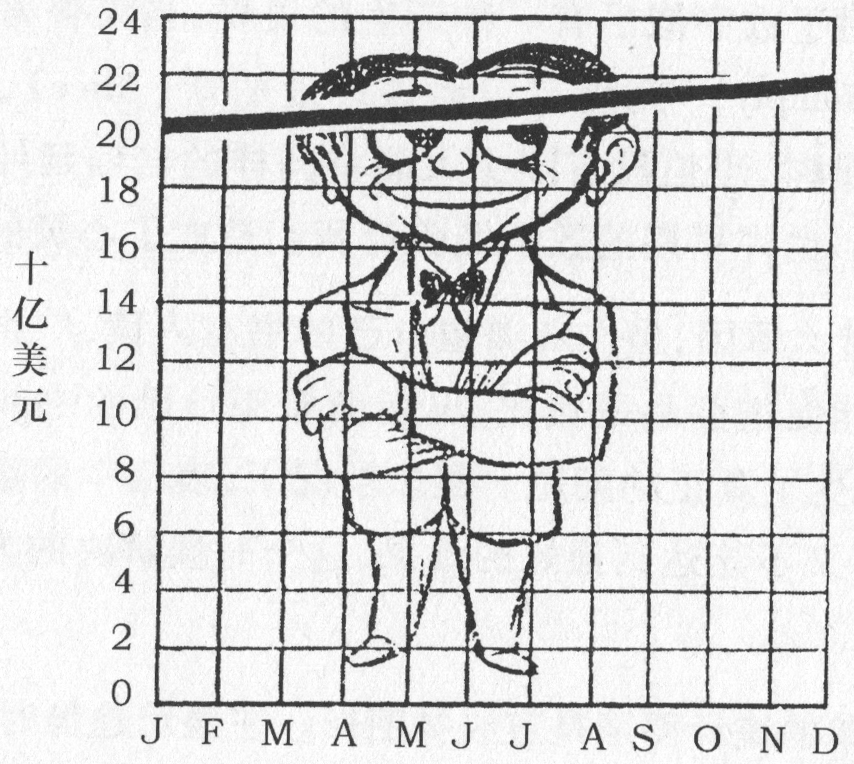
\includegraphics[width=0.7\textwidth]{c4.case.line.income.01.png}
  \end{figure}
\end{frame}

\begin{frame}
  \frametitle{案例 | 纵轴 | 国民收入}
  \begin{block}{解析}
    \begin{itemize}
      \item 图清晰地显示了一年来的变化,而且变化是逐月反映出来的。
      \item 能看出上涨趋势,但却并不振奋人心。
      \item 传递信息的目的达到了,但缺乏渲染的效果(用于辩论、推销、推动……)。
    \end{itemize}
  \end{block}
  \pause
  \begin{block}{原因}
    \begin{itemize}
      \item 纵轴从原点即“0”开始
      \item 整张图形是按比例绘制的
    \end{itemize}
  \end{block}
\end{frame}

\begin{frame}
  \frametitle{案例 | 纵轴 | 国民收入}
  \begin{block}{抹去图形的底部}
    数据是相同的,所以图形也相同,除了图形给人留下的印象不同之外,没有进行任何的伪造。
  \end{block}
  \vspace{-0.5em}
  \begin{figure}
    \centering
    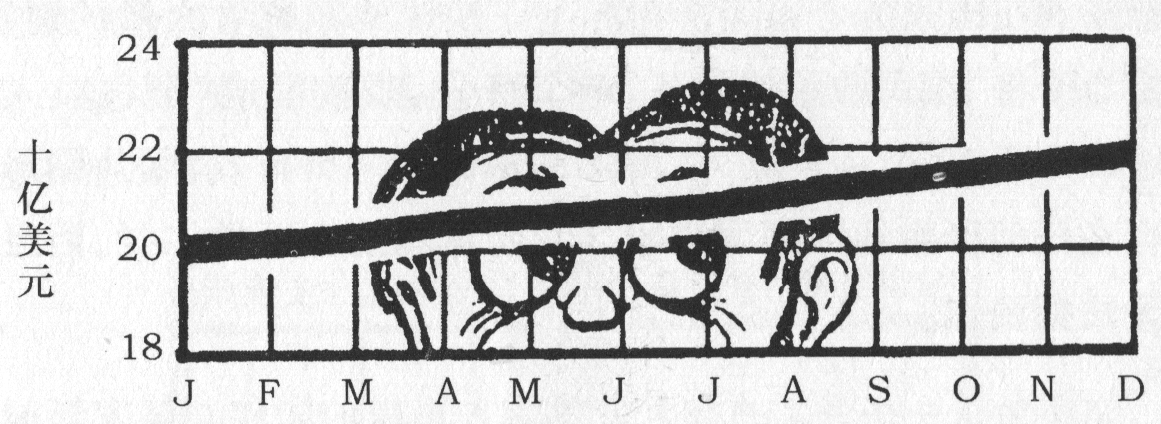
\includegraphics[width=0.9\textwidth]{c4.case.line.income.02.png}
  \end{figure}
  \pause
  \vspace{-0.5em}
  \begin{block}{解析}
    眼睛不能“理解”被抹去的部分,这才导致微小的上升最终变成了惊人的增长。
  \end{block}
\end{frame}

\begin{frame}
  \frametitle{案例 | 纵轴 | 国民收入}
  \begin{block}{改变横坐标与纵坐标的比例关系}
    将纵坐标的每一个刻度缩减为原来的1/10即可,没有人规定不能这么做,而这将会产生一张更加完美的图形——使朴实的10\%的增长率看上去比100\%的增长率更让人振奋。
  \end{block}
  \vspace{-0.5em}
  \begin{figure}
    \centering
    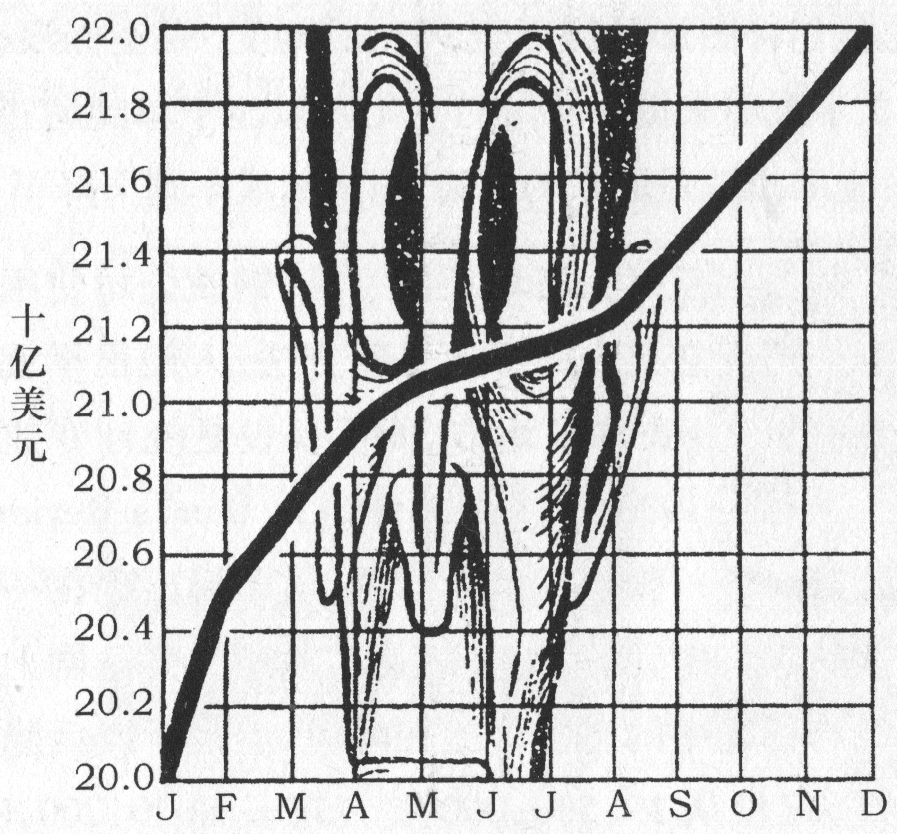
\includegraphics[width=0.5\textwidth]{c4.case.line.income.03.png}
  \end{figure}
\end{frame}

\begin{frame}
  \frametitle{案例 | 纵轴 | 国民收入}
  \begin{block}{令人惊奇的图形}
    \begin{itemize}
      \item 任何看到这幅图的人都会强烈地感觉到在国家的各条经济命脉上正快速地积累着大量的财富。
      \item 这相当于将“国民收入增长了10个百分点”改写成了“国民收入惊人地攀升了10个百分点”。
      \item 显然图形比文字更有效,因为图形中不存在任何形容词和副词来破坏它所具有的客观性幻觉,而且谁也无法指责你。
    \end{itemize}
  \end{block}
\end{frame}

\begin{frame}
  \frametitle{案例 | 纵轴 | 新闻发言人对企业经营业绩的操作}
  \begin{block}{“灰姑娘”到“白雪公主”的蜕变}
    \begin{figure}
      \centering
      \visible<1->{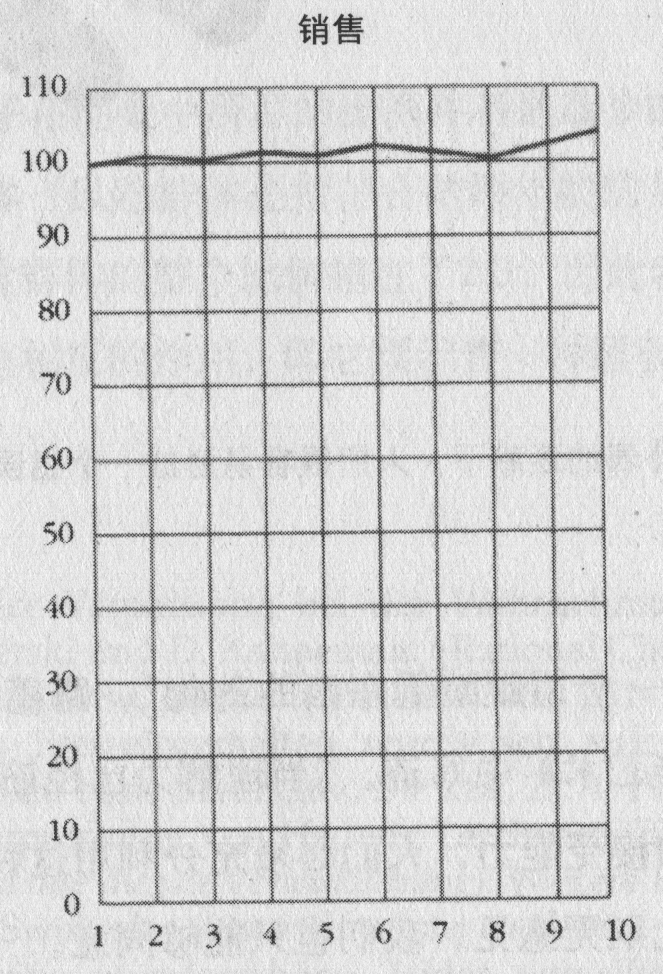
\includegraphics[width=0.22\textwidth]{c4.case.line.company.01.png}}
      \visible<2->{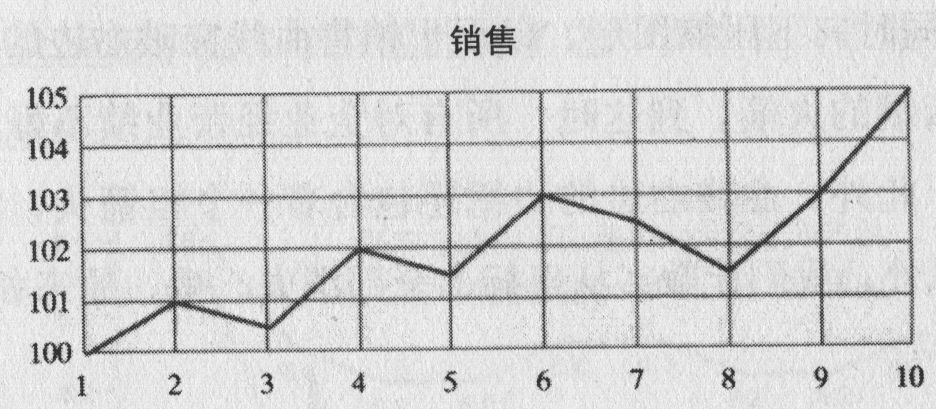
\includegraphics[width=0.28\textwidth]{c4.case.line.company.02.png}}
      \visible<3->{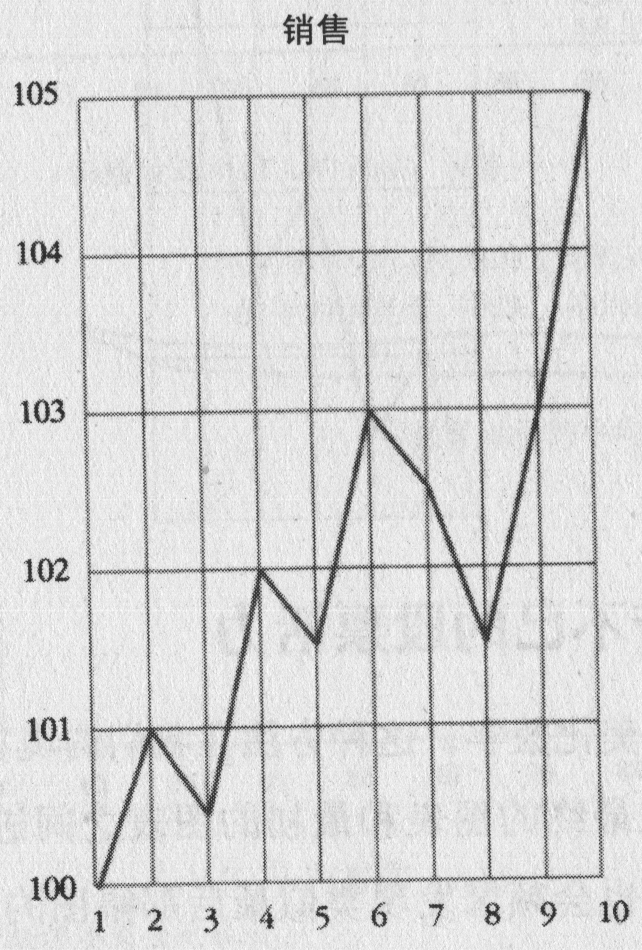
\includegraphics[width=0.22\textwidth]{c4.case.line.company.03.png}}
      \visible<4->{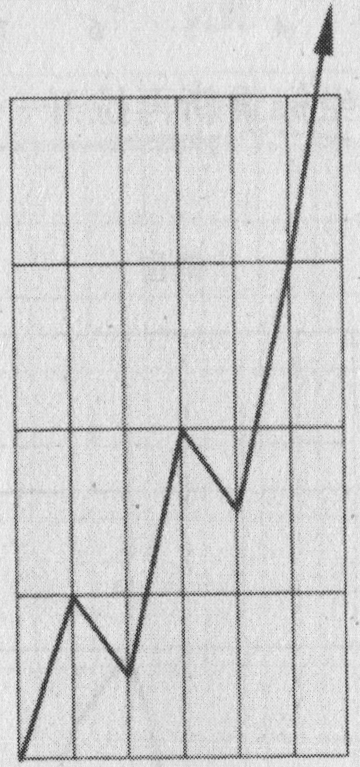
\includegraphics[width=0.155\textwidth]{c4.case.line.company.04.png}}
    \end{figure}
  \end{block}
\end{frame}

\begin{frame}
  \frametitle{案例 | 纵轴 | 政府支出}
  \begin{figure}
    \centering
    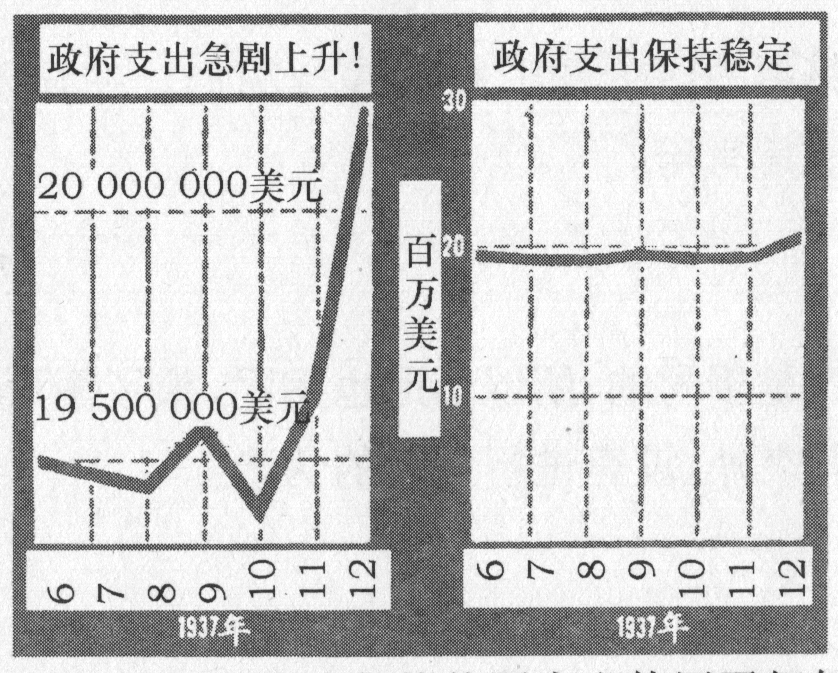
\includegraphics[width=0.58\textwidth]{c4.case.line.out.01.png}
  \end{figure}
  \vspace{-1em}
  \begin{block}{vs.}
    \begin{itemize}
      \item 保持稳定:折线客观地反映了4\%的增长率
      \item 急剧上升:折线从底部激增到顶端,将原本仅仅4\%的增长率描绘的仿佛是400\%
    \end{itemize}
  \end{block}
\end{frame}

\begin{frame}
  \frametitle{案例 | 纵轴 | 标致汽车的广告}
  \begin{figure}
    \centering
    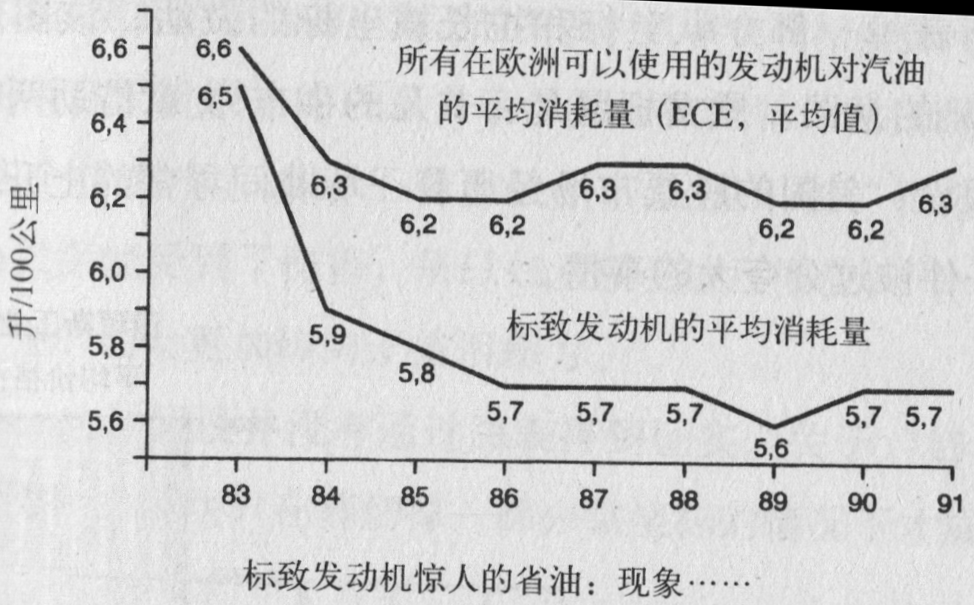
\includegraphics[width=0.48\textwidth]{c4.case.line.car.01.png}\quad
    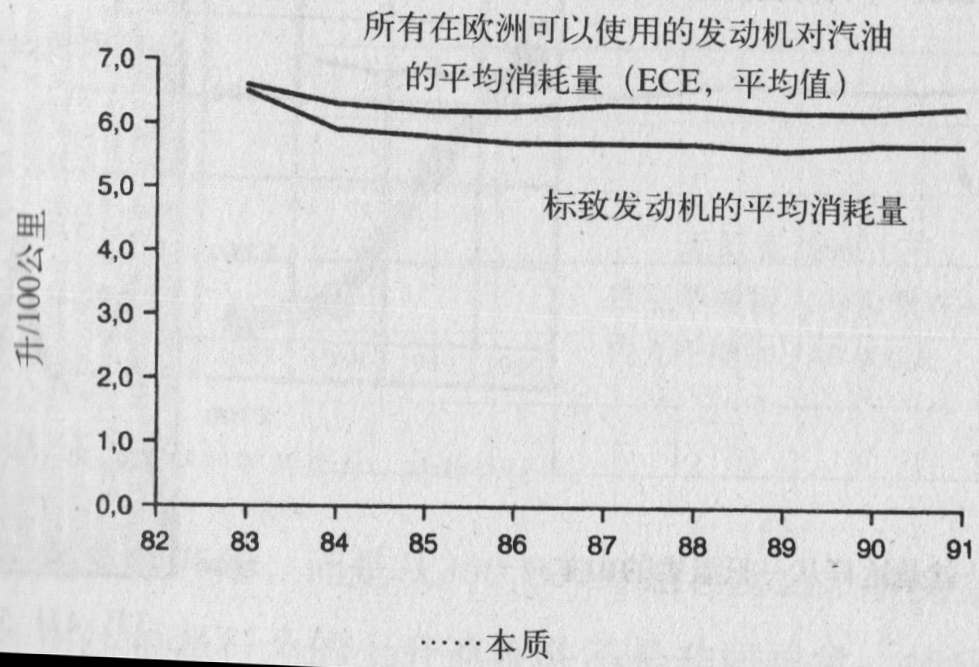
\includegraphics[width=0.43\textwidth]{c4.case.line.car.02.png}
  \end{figure}
\end{frame}

\begin{frame}
  \frametitle{案例 | 纵轴 | 美国道琼斯股票指数}
  \begin{block}{非凡的牛市!?}
    \begin{figure}
      \centering
      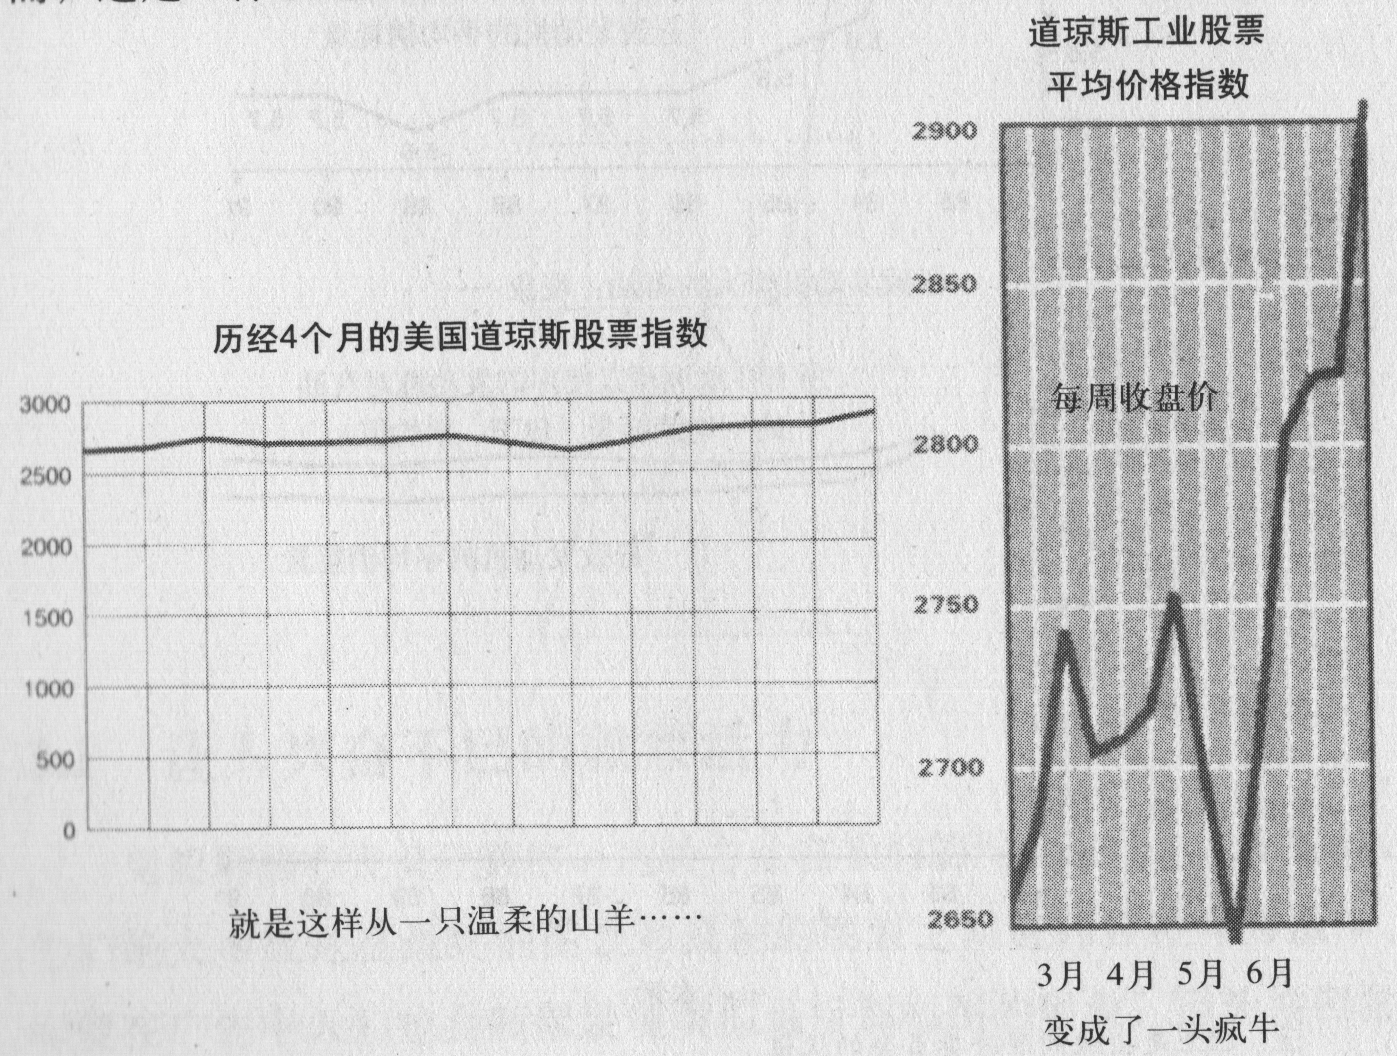
\includegraphics[width=0.7\textwidth]{c4.case.line.shock.01.png}
    \end{figure}
  \end{block}
\end{frame}

\begin{frame}
  \frametitle{案例 | 纵轴 | 妇女和犯罪}
  \begin{block}{妇女更加倾向于使用暴力?}
    \begin{figure}
      \centering
      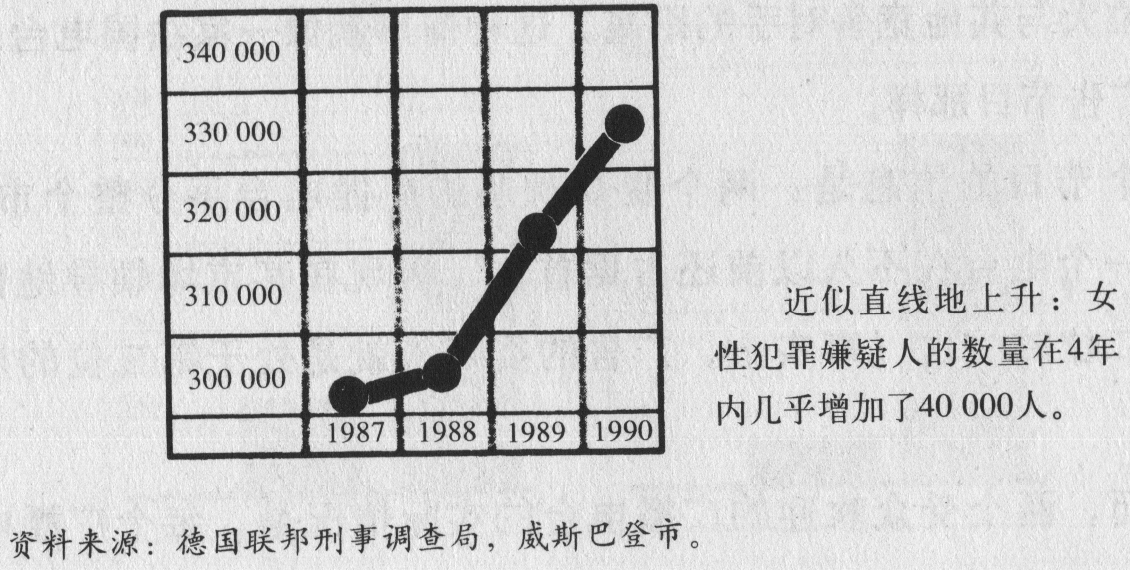
\includegraphics[width=0.68\textwidth]{c4.case.line.woman.01.png}
    \end{figure}
    \vspace{-1em}
    \pause
    从300000人上升到335000人,标志着4年内上升了11.7\%。或者说,平均每年的犯罪增长率不到3\%。\\
    \vspace{0.2em}
如果不是从300000开始,而是从零开始,那么,事实立即就会很清楚:女性违法犯罪行为的上升速度并不是非同寻常,相反还落后于一般刑事犯罪的上升幅度。也就是说,与男人相比,妇女并不容易表现得暴怒与粗暴,而是表现出平和与友好。
  \end{block}
\end{frame}

\begin{frame}
  \frametitle{案例 | 纵轴 | 柱状图}
  \begin{block}{一个被截短的柱状图与被截短的折线图实乃一丘之貉}
  \begin{figure}
    \centering
    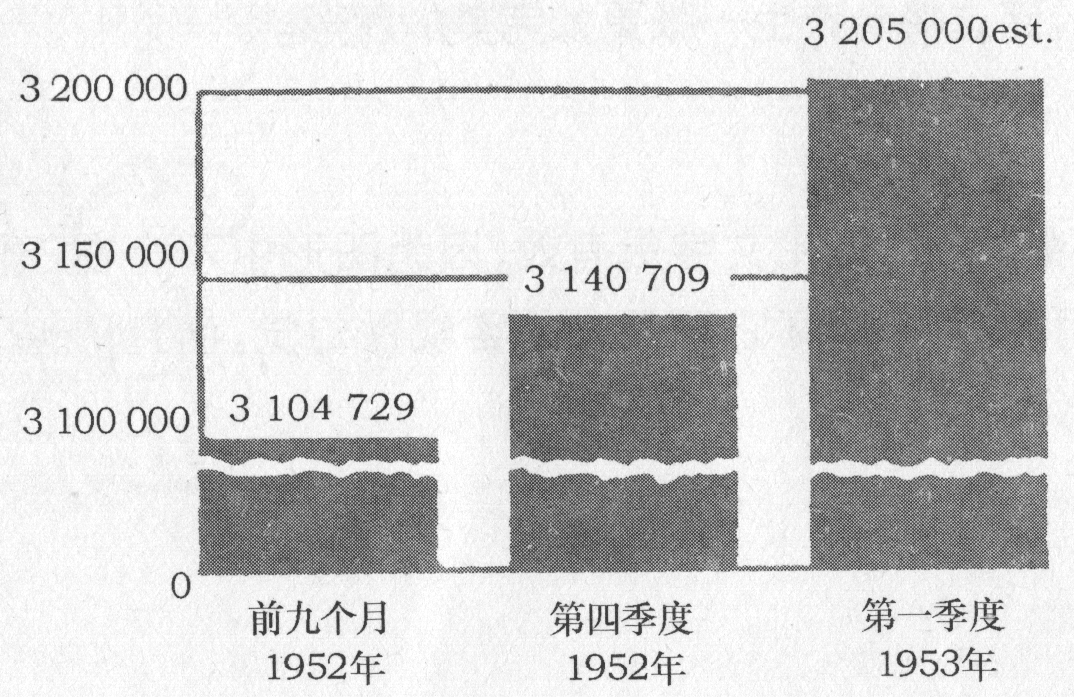
\includegraphics[width=0.9\textwidth]{c4.case.line.bar.01.png}
  \end{figure}
  \end{block}
\end{frame}

\begin{frame}
  \frametitle{案例 | 纵轴 | 德意志银行的顾客发展演变过程}
  \begin{figure}
    \centering
    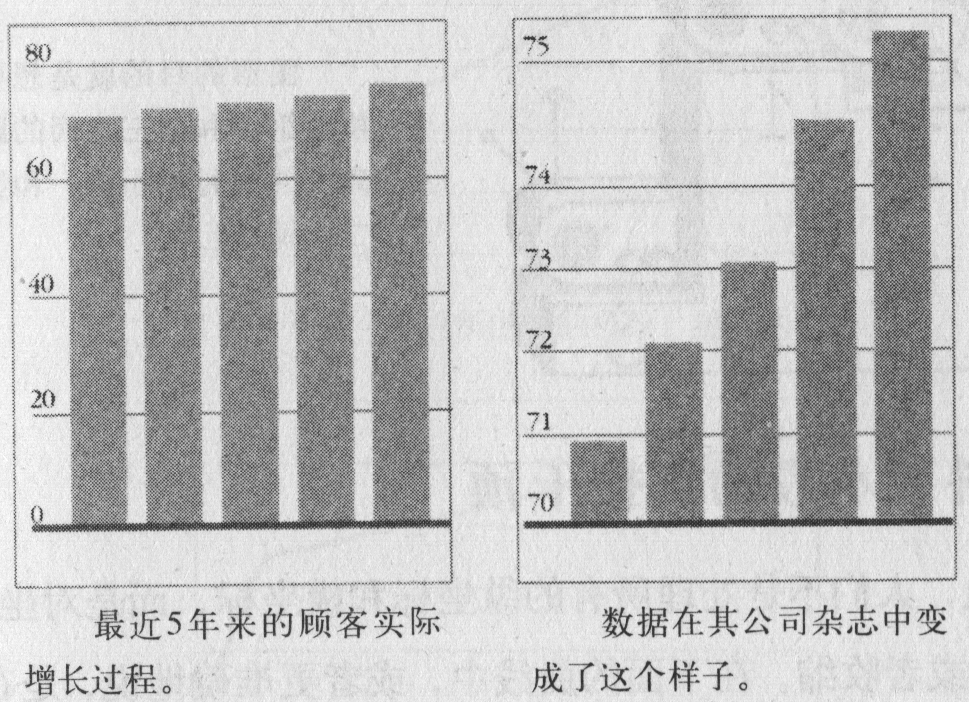
\includegraphics[width=0.5\textwidth]{c4.case.line.bank.01.png}\quad
    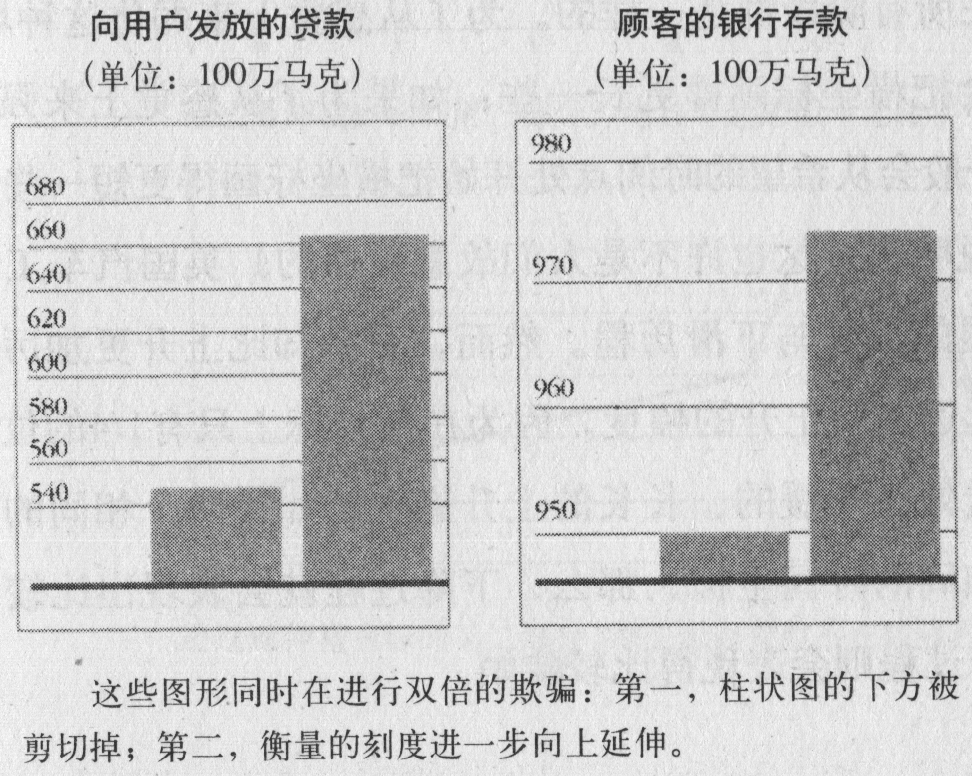
\includegraphics[width=0.46\textwidth]{c4.case.line.bank.02.png}
  \end{figure}
\end{frame}

\subsection{操作横轴}
\begin{frame}
  \frametitle{案例 | 横轴 | 延伸横坐标}
  \begin{block}{对坐标的一部分进行延伸或者收缩}
    \begin{itemize}
      \item<1-> 在直线中,绝对增长在所有阶段都是一样的。
      \item<2-> 为了从感觉上来弱化这种增长趋势,人们一般会把横坐标画得更长一些。
      \item<3-> 如果为了从感觉上来强化这种增长,人们一般会从希望的时间点处开始把横坐标画得更短一些。
    \end{itemize}
    \begin{figure}
      \centering
      \visible<1->{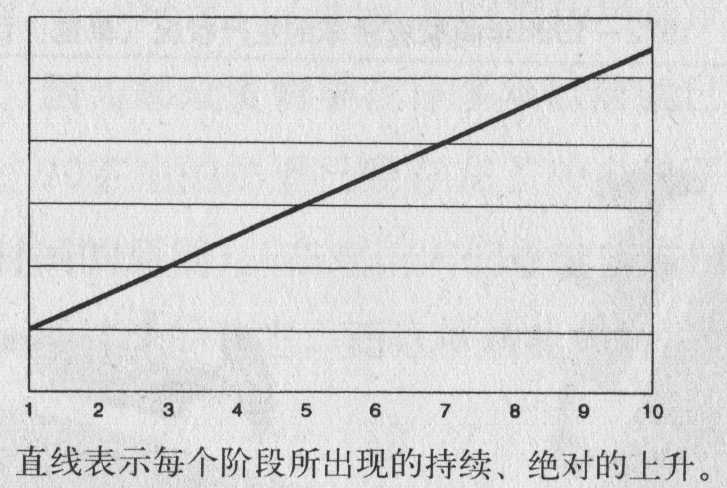
\includegraphics[width=0.3\textwidth]{c4.case.line.axis.01.png}}
      \visible<2->{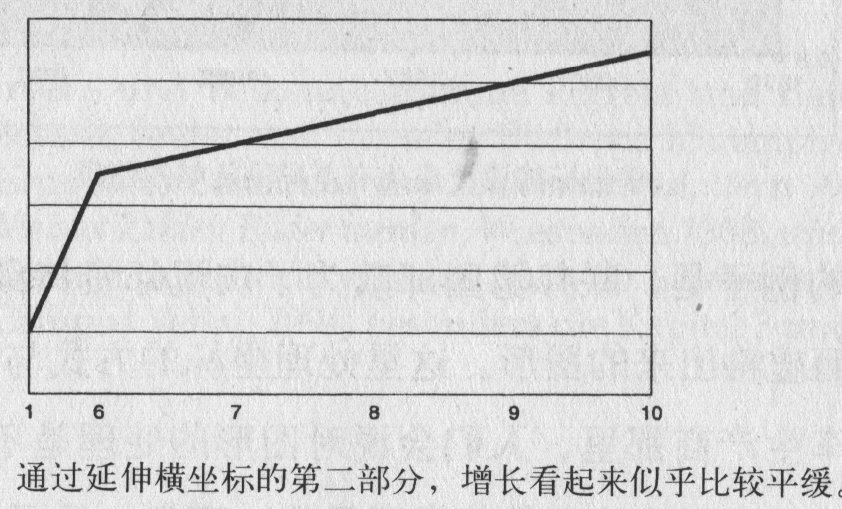
\includegraphics[width=0.33\textwidth]{c4.case.line.axis.02.png}}
      \visible<3->{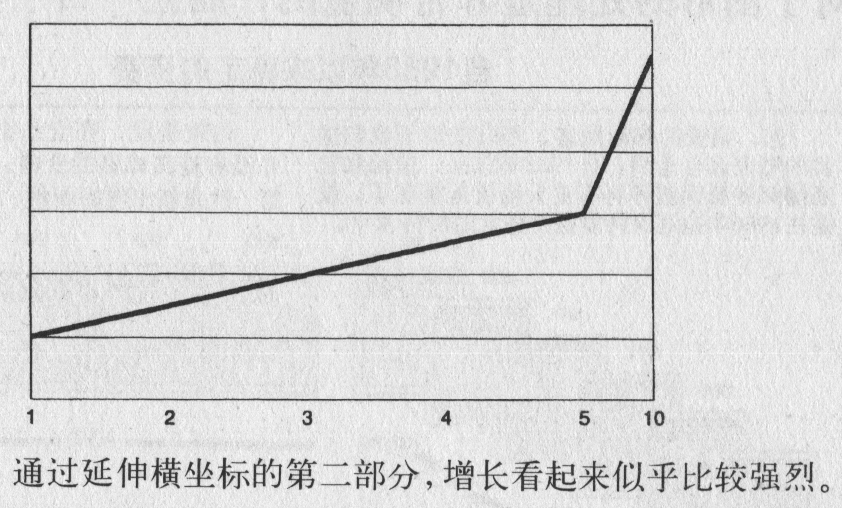
\includegraphics[width=0.33\textwidth]{c4.case.line.axis.03.png}}
    \end{figure}
  \end{block}
\end{frame}

\begin{frame}
  \frametitle{案例 | 横轴 | 英国汽车工业}
  \begin{block}{1972~1988年发展的上升与下滑历程}
    \begin{figure}
      \centering
      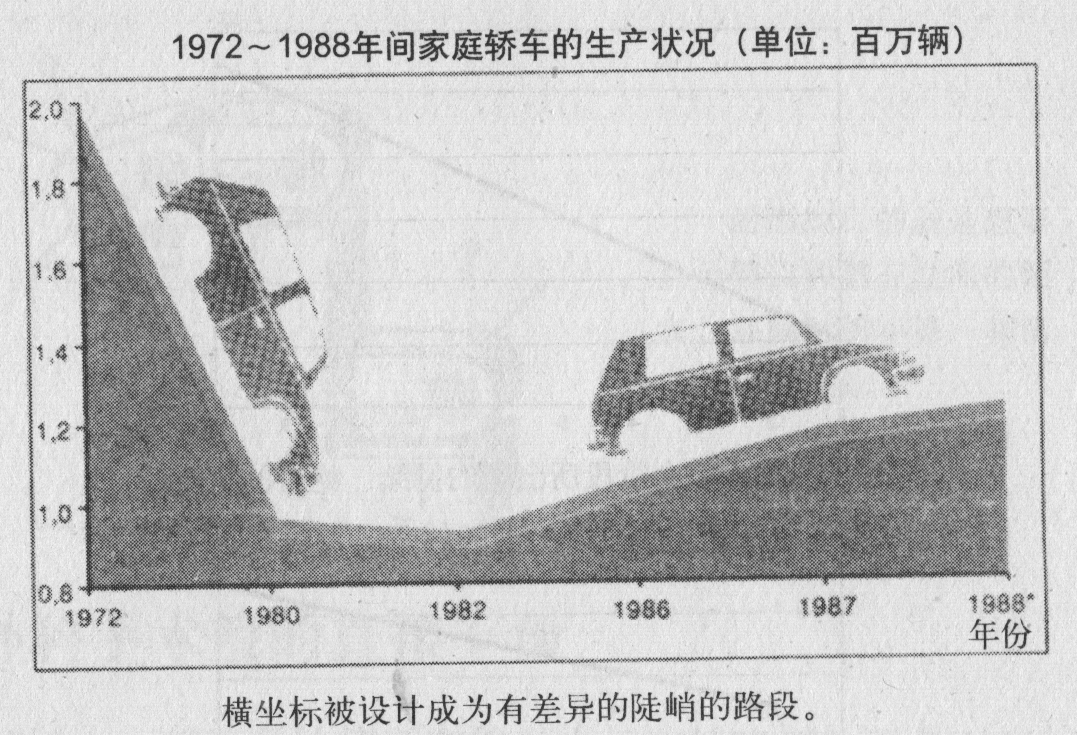
\includegraphics[width=0.8\textwidth]{c4.case.line.car.03.png}
    \end{figure}
  \end{block}
\end{frame}

\begin{frame}
  \frametitle{案例 | 横轴 | 联邦德国的邮政资费}
  \begin{block}{邮资持续不变的假象}
    \begin{figure}
      \centering
      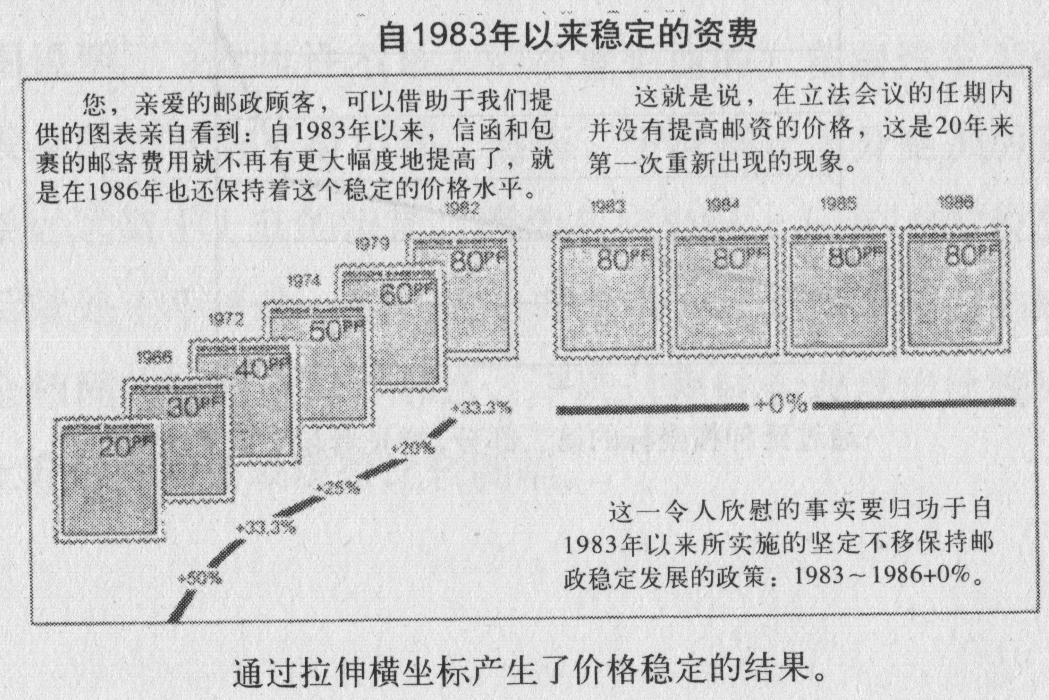
\includegraphics[width=0.8\textwidth]{c4.case.line.stamp.01.png}
    \end{figure}
  \end{block}
\end{frame}

\subsection{增减信息}
\begin{frame}
  \frametitle{案例 | 信息 | 自我宣传}
  \begin{block}{广告代理机构宣传自己的广告}
    \begin{figure}
      \centering
      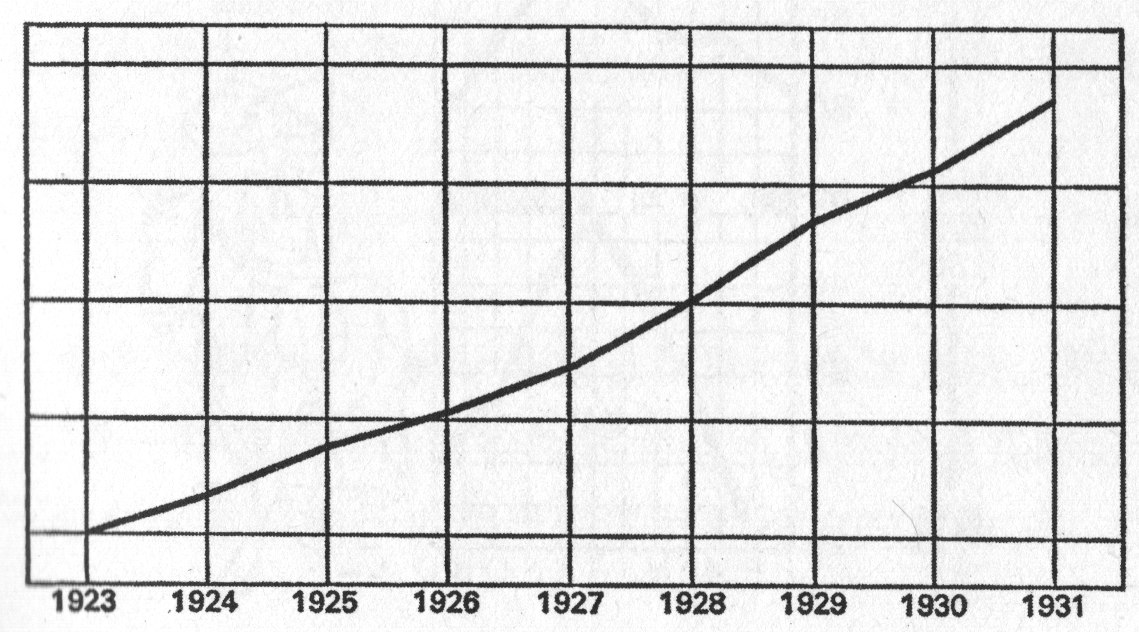
\includegraphics[width=0.9\textwidth]{c4.case.line.other.01.png}
    \end{figure}
  \end{block}
\end{frame}

\begin{frame}
  \frametitle{案例 | 信息 | 自我宣传}
  \begin{block}{广告代理机构宣传自己的广告}
图中曲线意欲向人们显示这家广告公司年复一年惊人的发展趋势。但途中没有一个数字,这样一来,它既可以代表一个骇人的发展速度,每年翻番或增长几百万美金,又可以意味着在年十亿总收入的基础上,增加了一美元或两美元相对稳定的蛇状爬行。但仅从图上看,其发展速度让人印象深刻。
  \end{block}
\end{frame}

\begin{frame}
  \frametitle{案例 | 信息 | 薄饼}
  \begin{block}{薄饼“在2分钟之内开始提供能量”}
    \begin{figure}
      \centering
      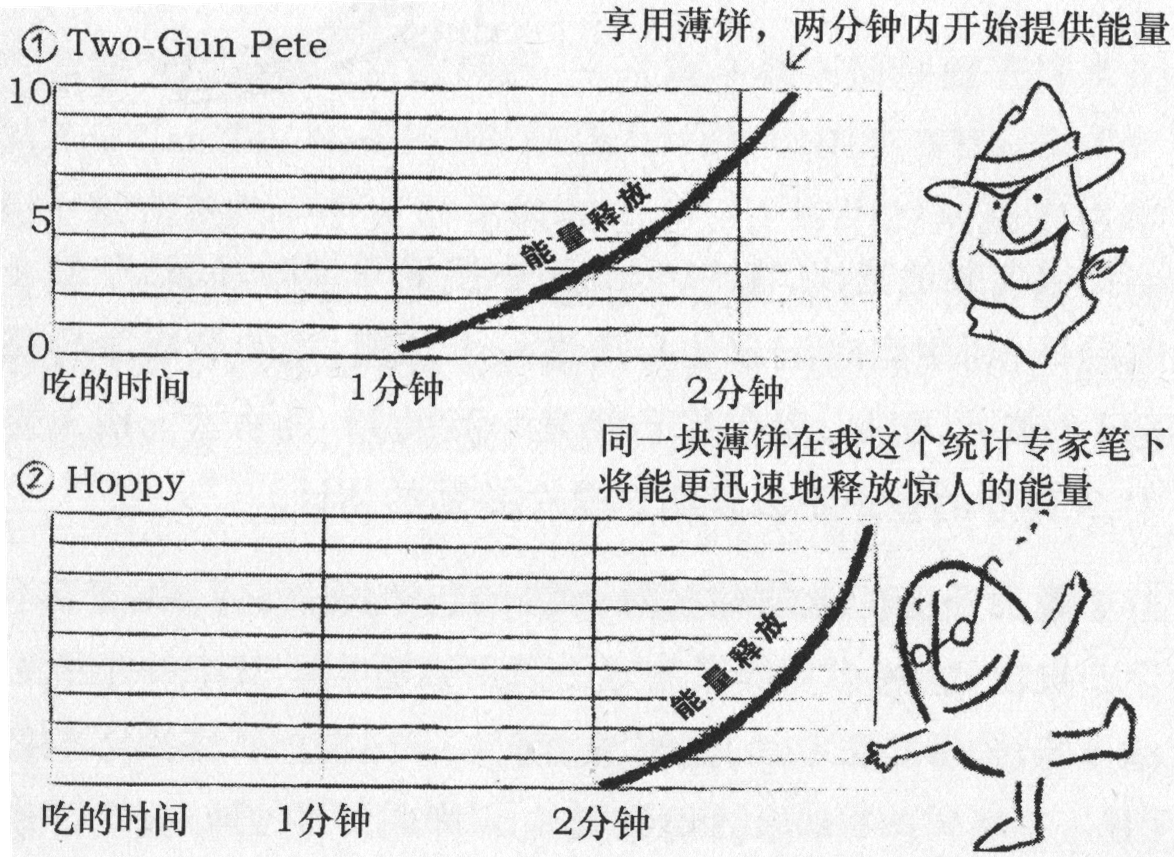
\includegraphics[width=0.8\textwidth]{c4.case.line.other.02.png}
    \end{figure}
  \end{block}
\end{frame}

\begin{frame}
  \frametitle{案例 | 信息 | 经济上升}
  \begin{block}{经济上升}
  \begin{figure}
    \centering
    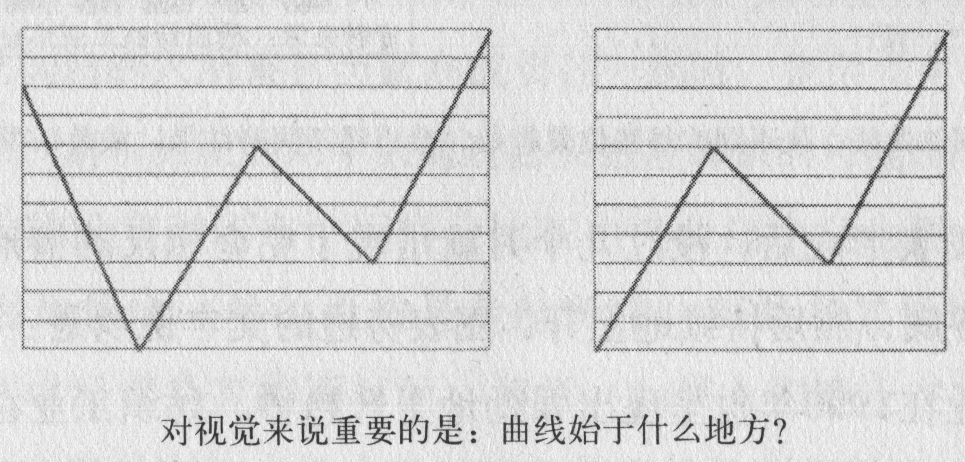
\includegraphics[width=0.9\textwidth]{c4.case.line.other.06.png}
  \end{figure}
  \end{block}
\end{frame}

\begin{frame}
  \frametitle{案例 | 信息 | “马屁精”}
  \begin{block}{使用相同的数据同时取悦共和党和民主党}
    \begin{figure}
      \centering
      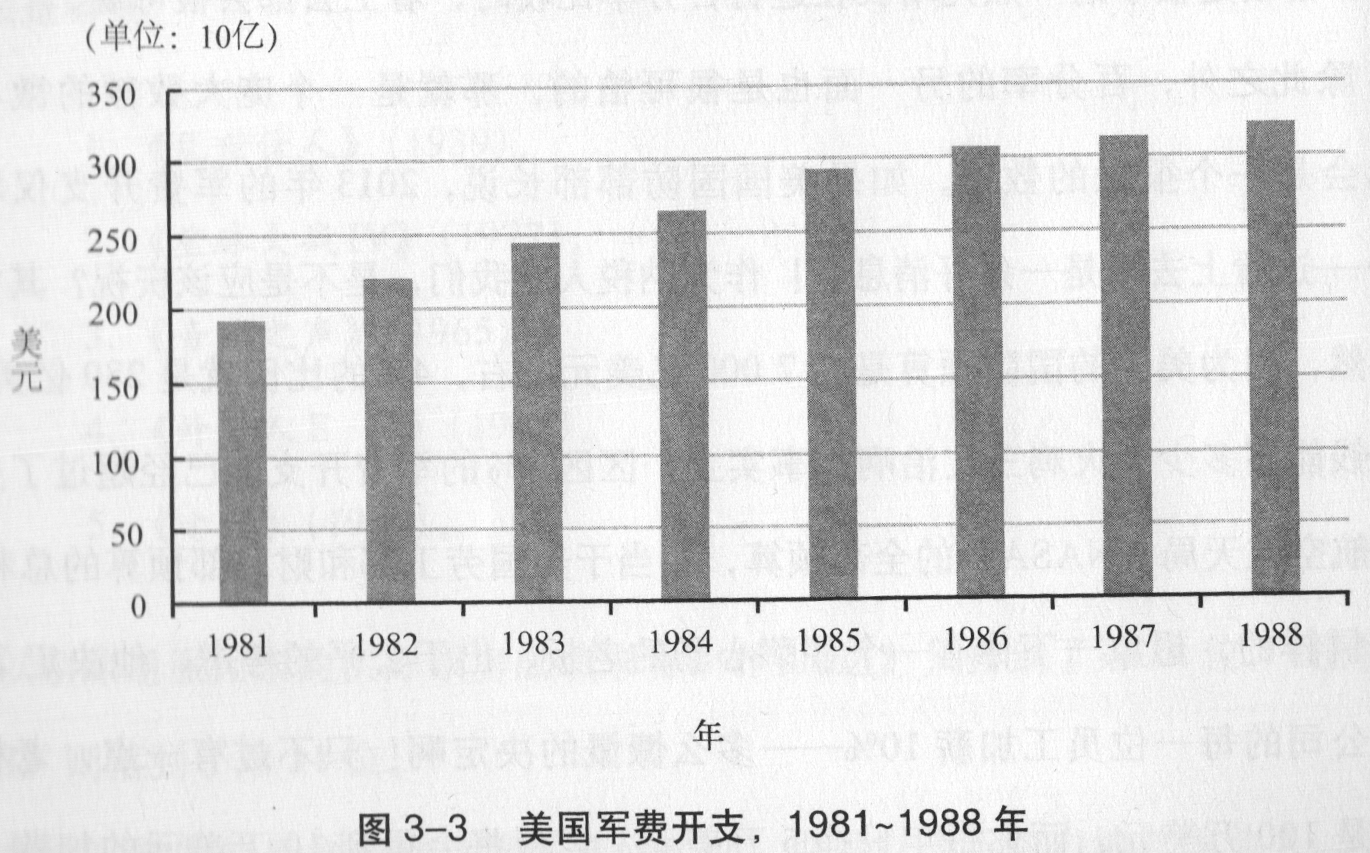
\includegraphics[width=0.51\textwidth]{c4.case.line.other.04.png}\quad
      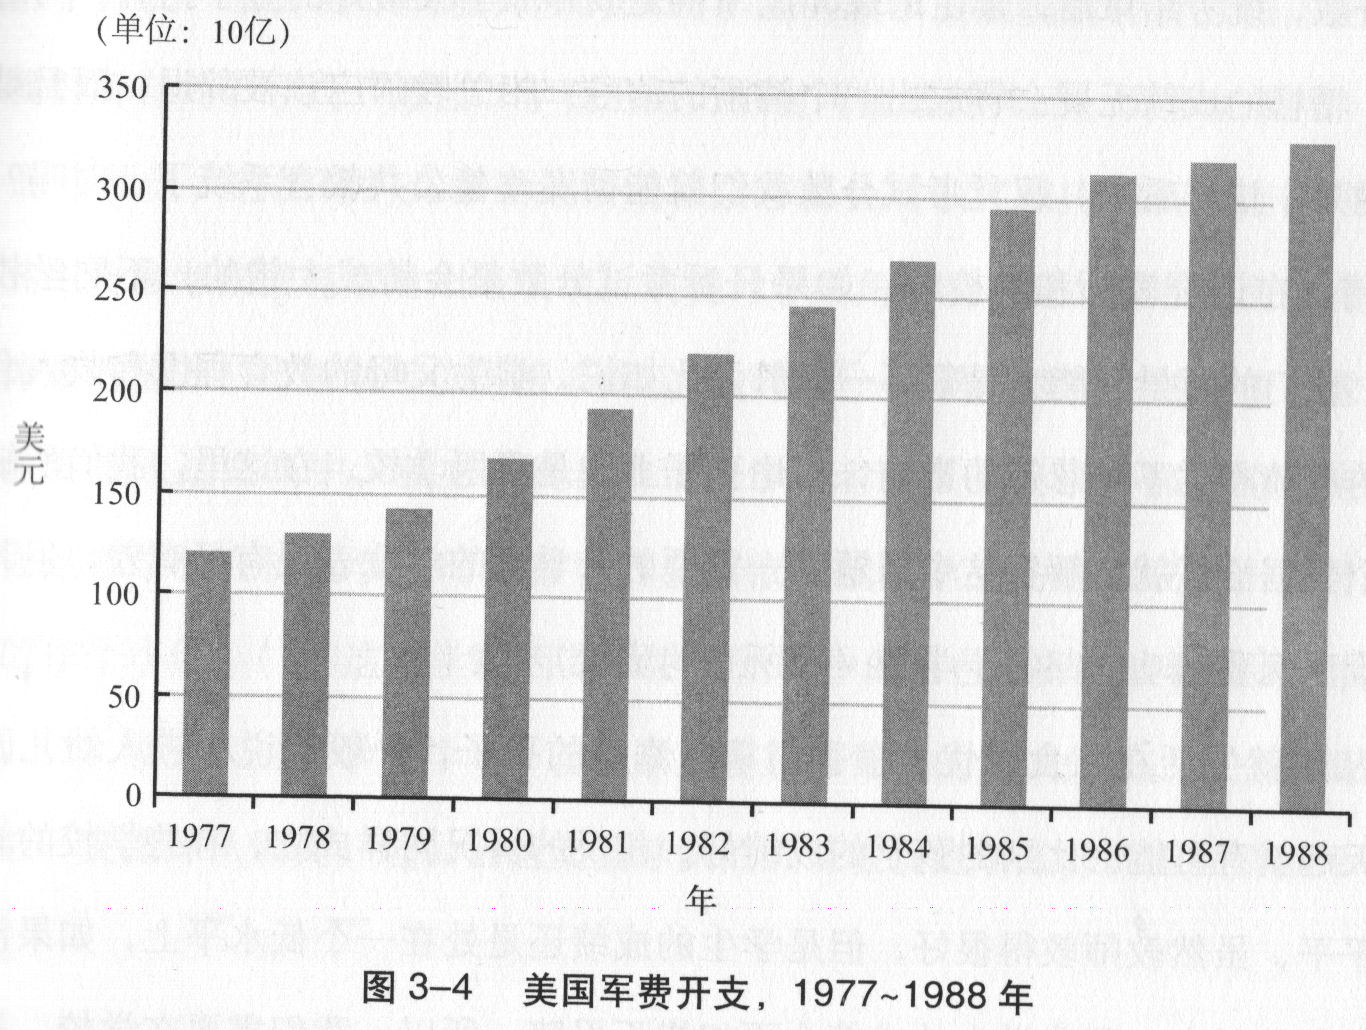
\includegraphics[width=0.42\textwidth]{c4.case.line.other.05.png}
    \end{figure}
  \end{block}
\end{frame}

\begin{frame}
  \frametitle{案例 | 信息 | 德国纺织工业}
  \begin{block}{德国纺织工业去向何方}
    \begin{figure}
      \centering
      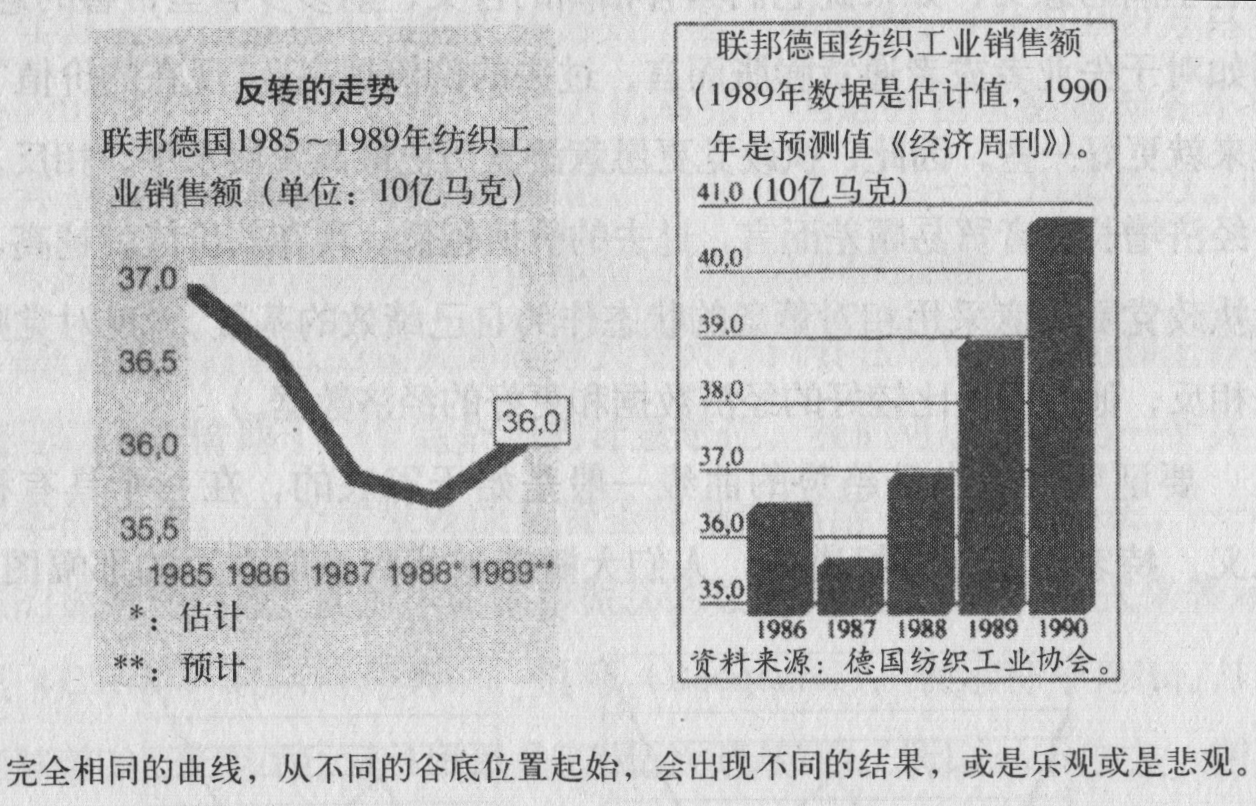
\includegraphics[width=0.9\textwidth]{c4.case.line.other.07.png}
    \end{figure}
  \end{block}
\end{frame}

\begin{frame}
  \frametitle{案例 | 信息 | 美国制造业}
  \begin{block}{美国制造业的完整故事}
    \begin{figure}
      \centering
      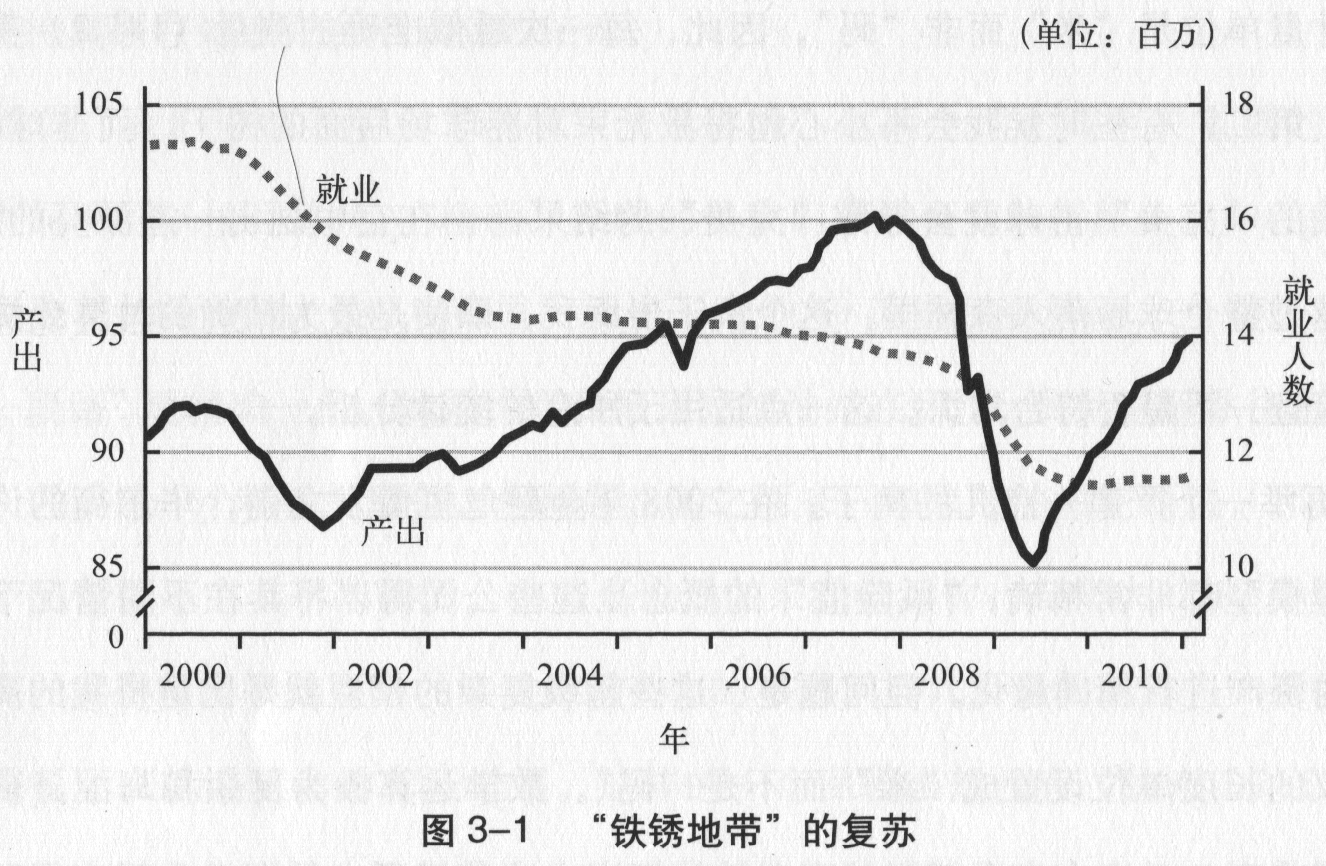
\includegraphics[width=0.9\textwidth]{c4.case.line.other.03.png}
    \end{figure}
  \end{block}
\end{frame}

\begin{frame}
  \frametitle{案例 | 信息 | 广播电台的市场份额}
  \begin{block}{双雄争霸 vs. 三足鼎立}
    \begin{figure}
      \centering
      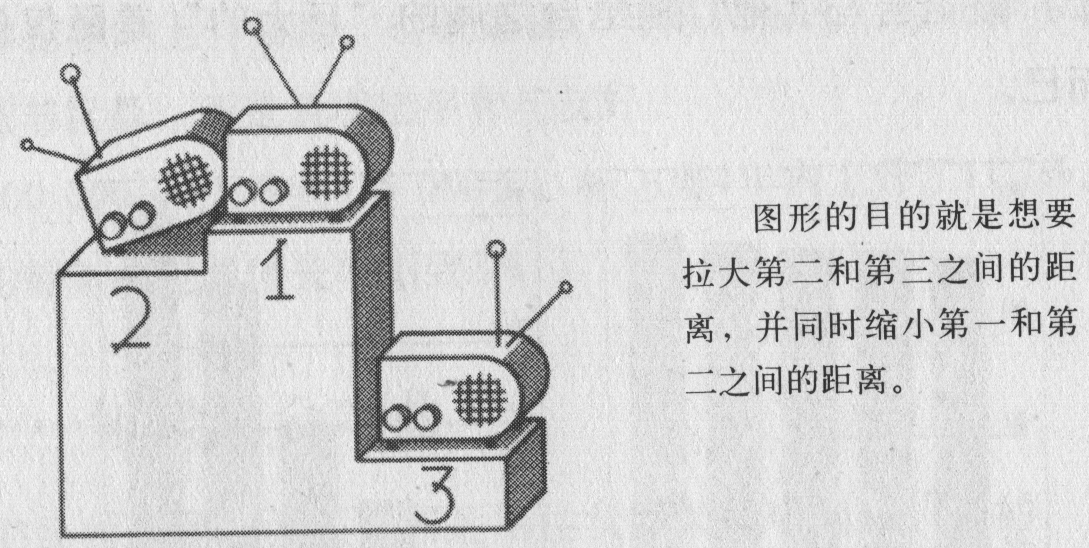
\includegraphics[width=0.7\textwidth]{c4.case.line.radio.01.png}
    \end{figure}
    \vspace{-1em}
    \pause
两个受欢迎的广播电台的实际情况是,每个广播电台都只拥有7\%的广播听众,而第三位的广播电台和其他广播电台拥有4\%的广播听众。换句话说,对于在广播电台做广告来说,每个广播电台都是一样的,没有一个广播电台能够控制并独占市场,受众最多的两个广播电台与其他广播电台之间的“巨大的”差距仅仅是一个幻象而已。
  \end{block}
\end{frame}

\subsection{趋势外推}
\begin{frame}
  \frametitle{案例 | 趋势 | 德国股份公司的收益}
  \begin{block}{一个过去的趋势在未来的10年得到了进一步的延续与升级}
    \begin{figure}
      \centering
      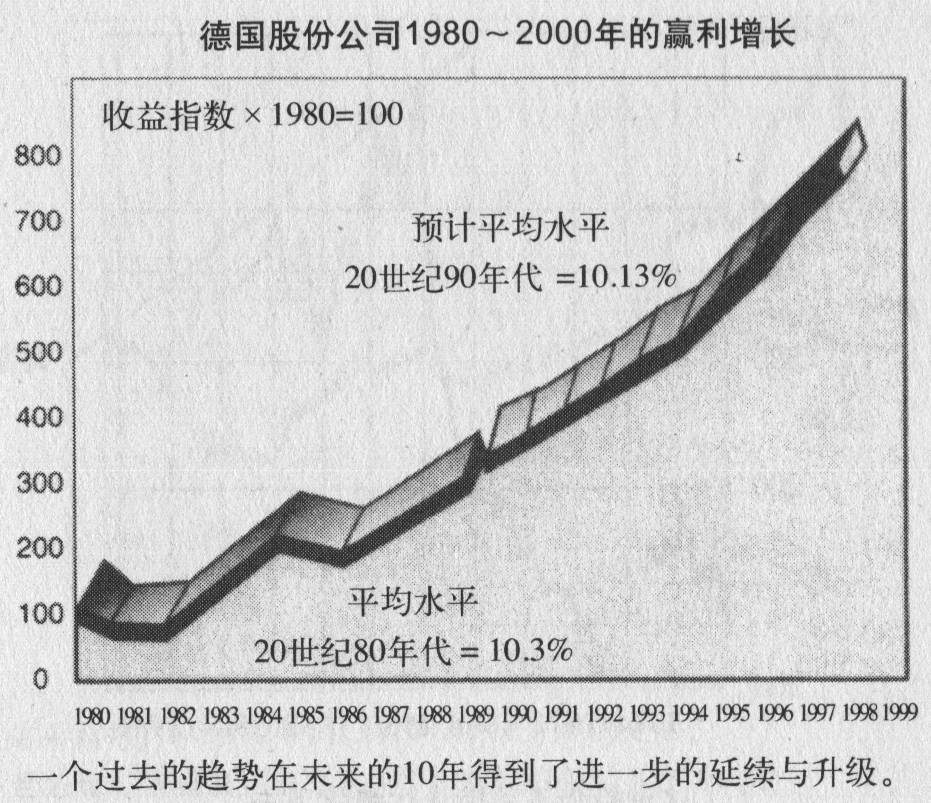
\includegraphics[width=0.6\textwidth]{c4.case.line.ten.01.png}
    \end{figure}
  \end{block}
\end{frame}

\begin{frame}
  \frametitle{案例 | 趋势 | 黄金价格}
  \begin{block}{黄金价格的未来趋势}
    \begin{figure}
      \centering
      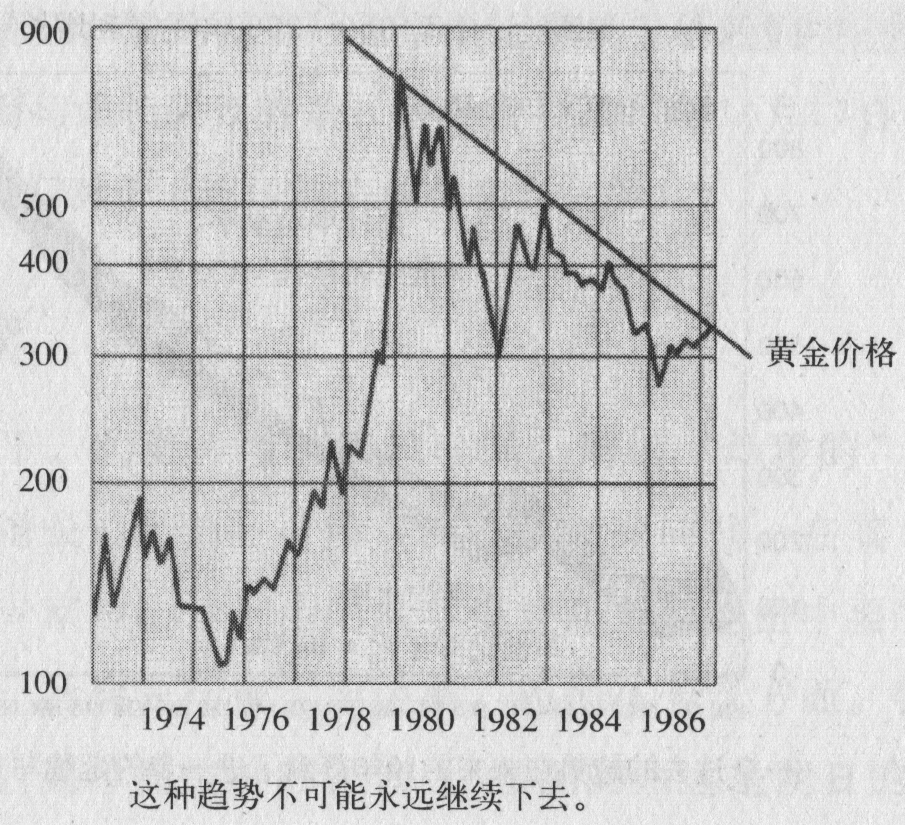
\includegraphics[width=0.6\textwidth]{c4.case.line.gold.01.png}
    \end{figure}
  \end{block}
\end{frame}

\begin{frame}
  \frametitle{案例 | 趋势 | 股指的走势}
  \begin{figure}
    \centering
    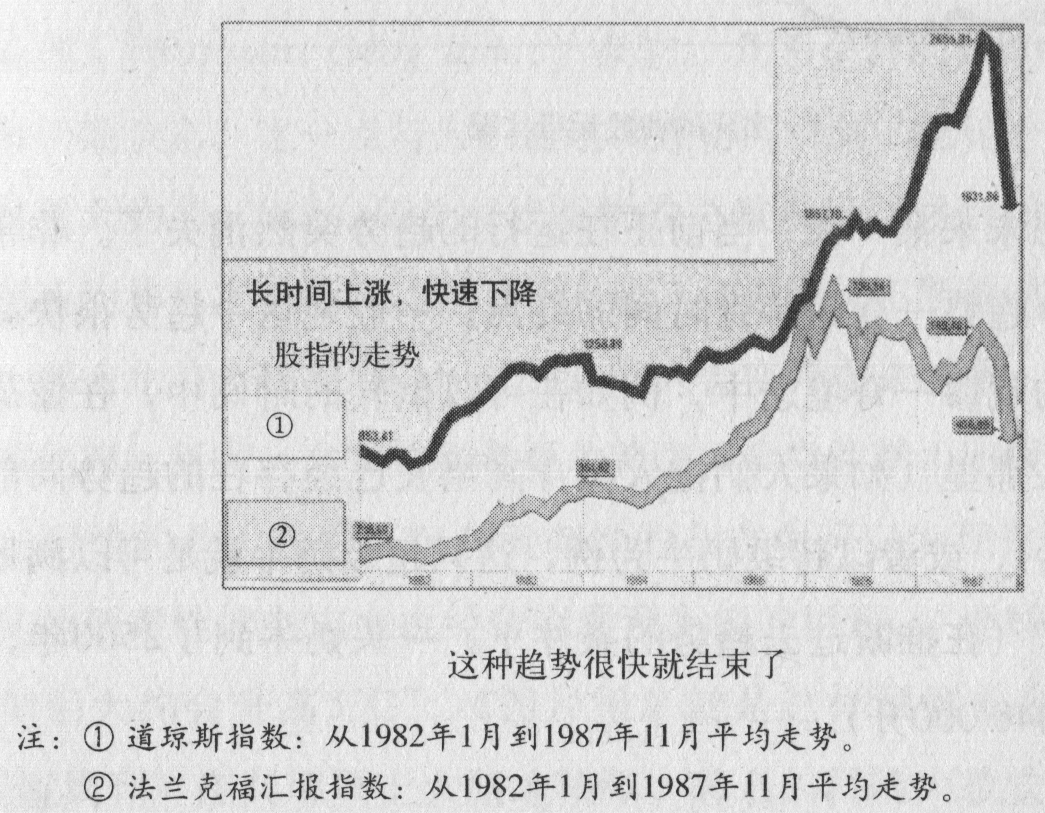
\includegraphics[width=0.43\textwidth]{c4.case.line.shock.02.png}\quad
    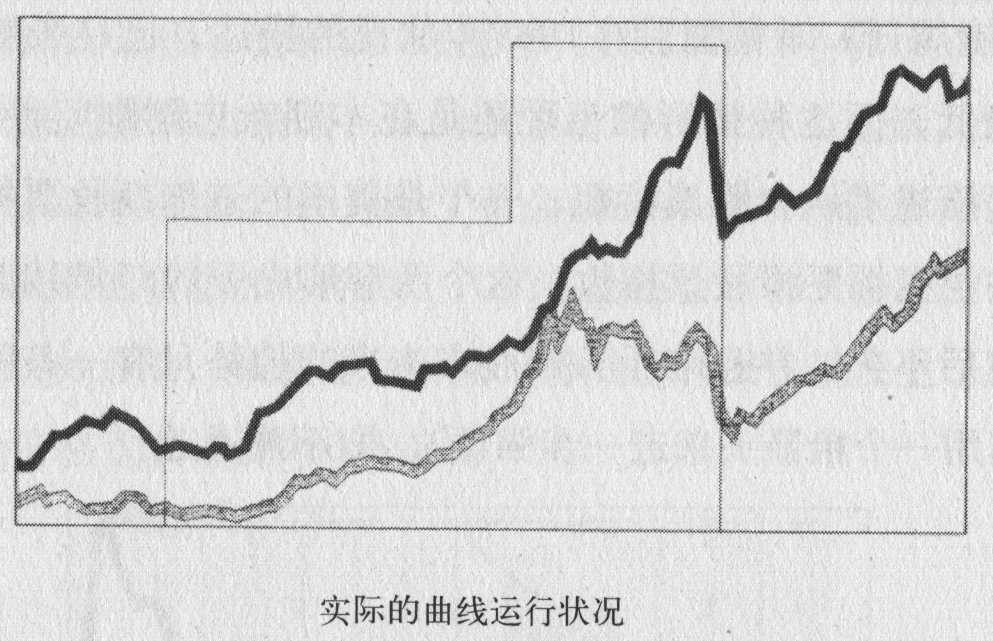
\includegraphics[width=0.52\textwidth]{c4.case.line.shock.03.png}
  \end{figure}
\end{frame}

\begin{frame}
  \frametitle{案例 | 趋势 | 艾滋病未来的发展趋势}
  \begin{figure}
    \centering
    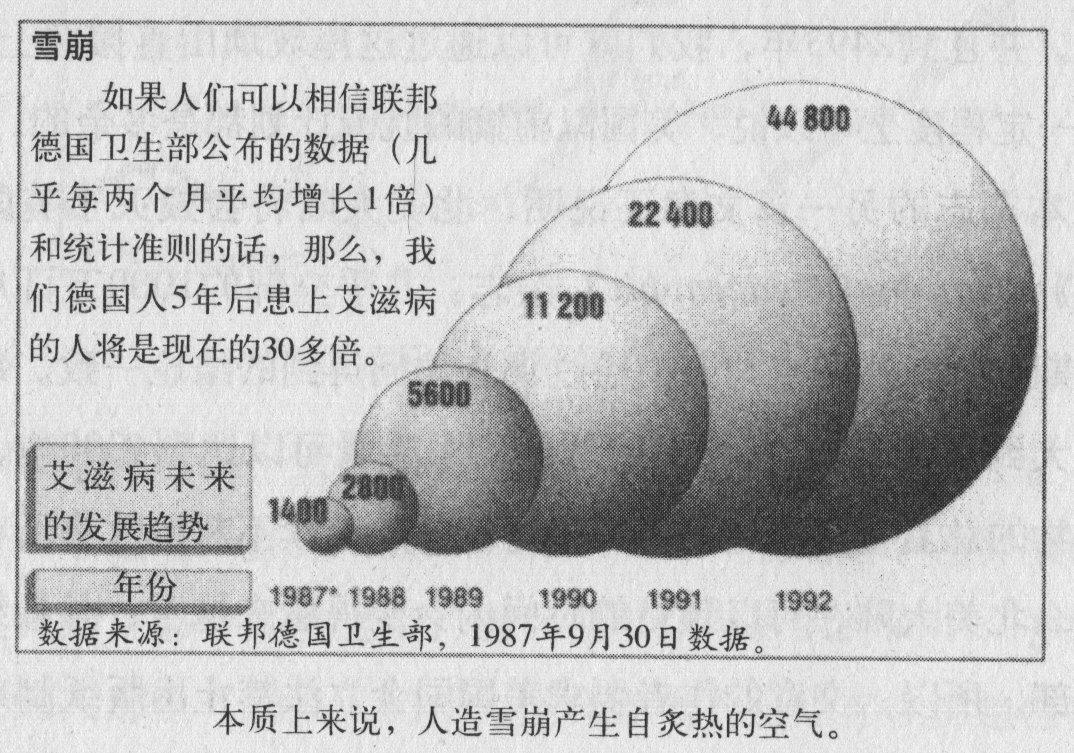
\includegraphics[width=0.9\textwidth]{c4.case.line.hiv.01.png}
  \end{figure}
\end{frame}

\begin{frame}
  \frametitle{案例 | 趋势 | “罗马俱乐部”的末日论}
  \begin{block}{农田需求}
    \begin{figure}
      \centering
      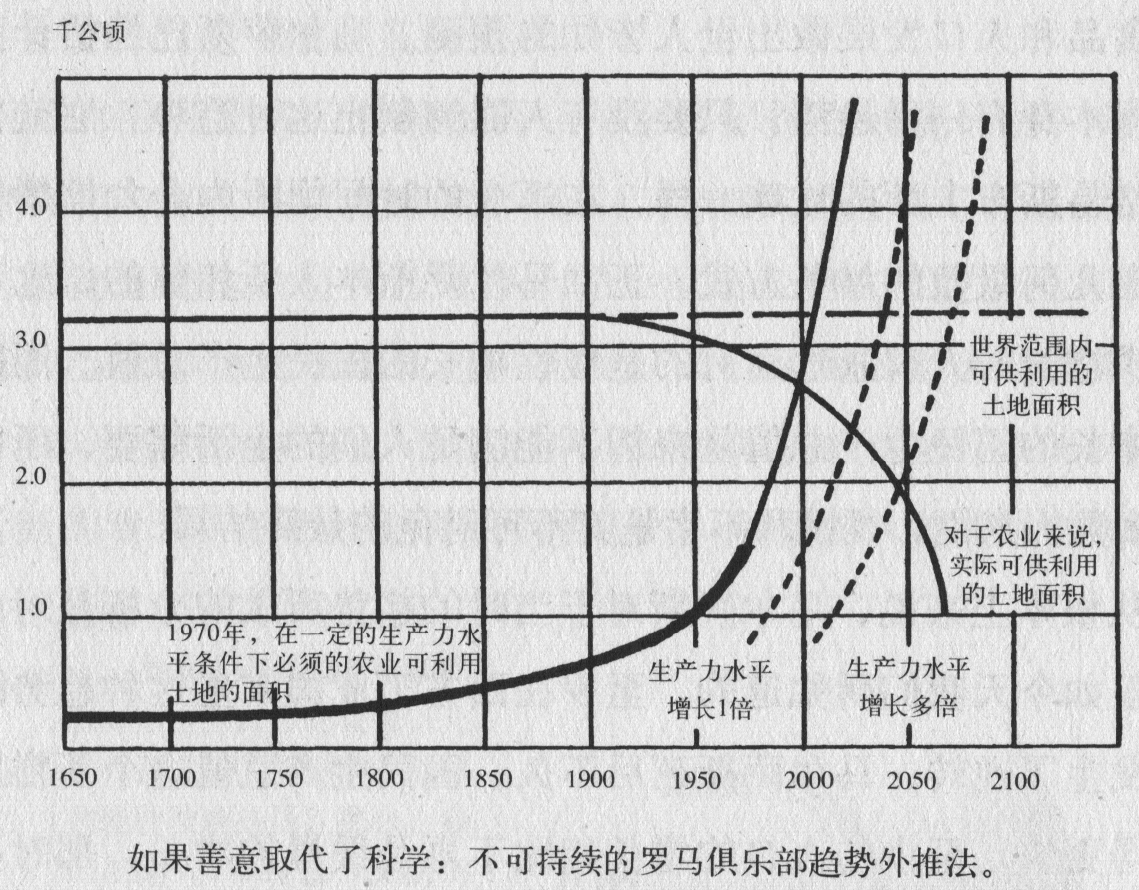
\includegraphics[width=0.7\textwidth]{c4.case.line.land.01.png}
    \end{figure}
  \end{block}
\end{frame}

\begin{frame}
  \frametitle{案例 | 趋势 | “罗马俱乐部”的末日论}
  \begin{block}{大气环境中的二氧化碳}
    \begin{figure}
      \centering
      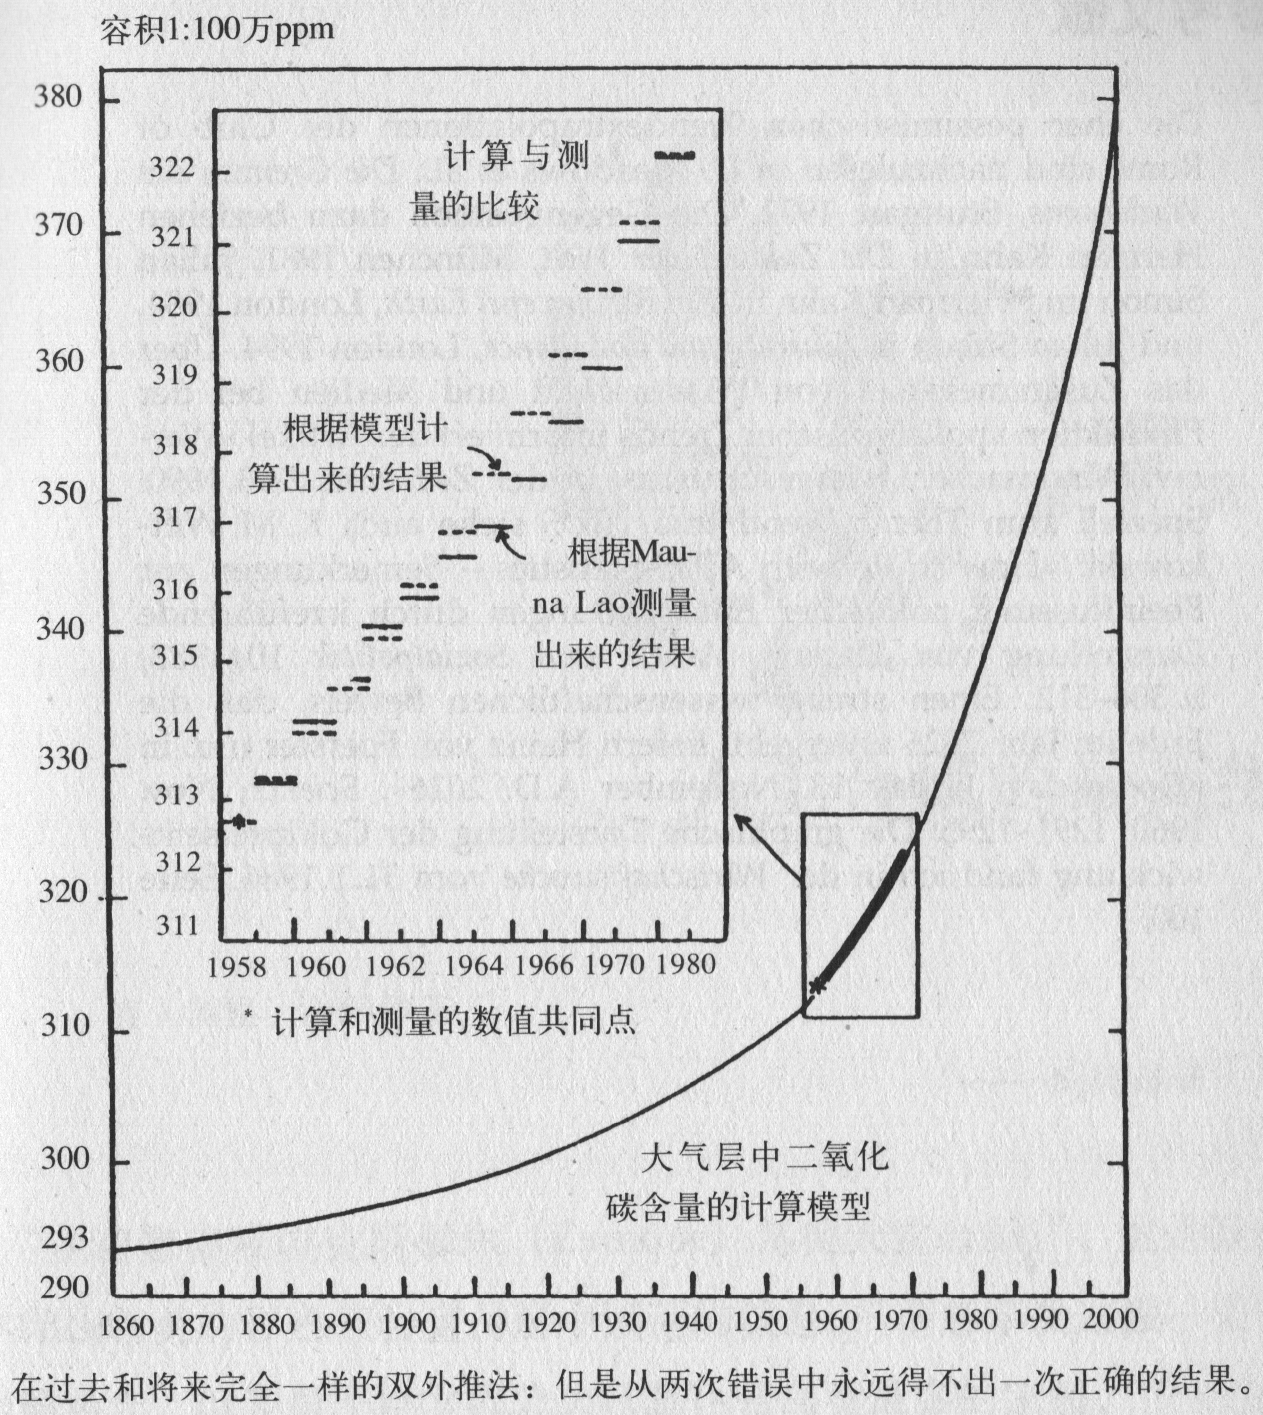
\includegraphics[width=0.48\textwidth]{c4.case.line.air.01.png}
    \end{figure}
  \end{block}
\end{frame}

\subsection{一维图形}
\begin{frame}
  \frametitle{案例 | 维度 | 引言}
  \begin{block}{形象图形}
    形象图形,又称为象形图,它的前身是普通的柱状图,在比较两种或两种以上事物某个方面的具体数量时,柱状图是一种便捷常用的方法。\\
但是柱状图也具有欺骗性:在描述单一物体时,柱体改变宽度的同时,长度也发生变化;在描述三维物体时,物体的体积又不容易进行比较,以上任何一种情况都提醒我们应该对柱状图保留一些怀疑。\\
  \end{block}
  \pause
  \begin{block}{双刃剑}
    \begin{itemize}
      \item 用一个小人来表示成千上万的人,一个钱袋或一堆硬币表示一千英镑或者百万美金,一篇牛肉表示明年牛肉的供应量,这些都是形象的图形表示。
      \item 由于这种图形非常吸引眼球,所以可以作为一种有用的工具,但同时它也能摇身一变,成为一个老练、狡猾而且成功的骗子。
    \end{itemize}
  \end{block}
\end{frame}

\begin{frame}
  \frametitle{案例 | 维度 | 工资}
  \begin{block}{目标}
    \begin{itemize}
      \item 比较两个数据——英国与罗坦提亚某工种公认的平均周工资,假设数值分别为30英镑和15英镑。
      \item 未说出的目的——说明英国工人比罗坦提亚工人的境况好得多(差距渲染得越大论据越充分)。
      \item 同时避免麻烦——希望你能从中推断出什么,或者留下一个夸张的印象,而作者又不会因此惹上麻烦。
    \end{itemize}
  \end{block}
  \pause
  \begin{block}{方法}
    \begin{itemize}
      \item 直接将数字打印出来
      \item 为了吸引注意,画出柱状图
    \end{itemize}
  \end{block}
\end{frame}

\begin{frame}
  \frametitle{案例 | 维度 | 工资}
  \begin{figure}
    \centering
    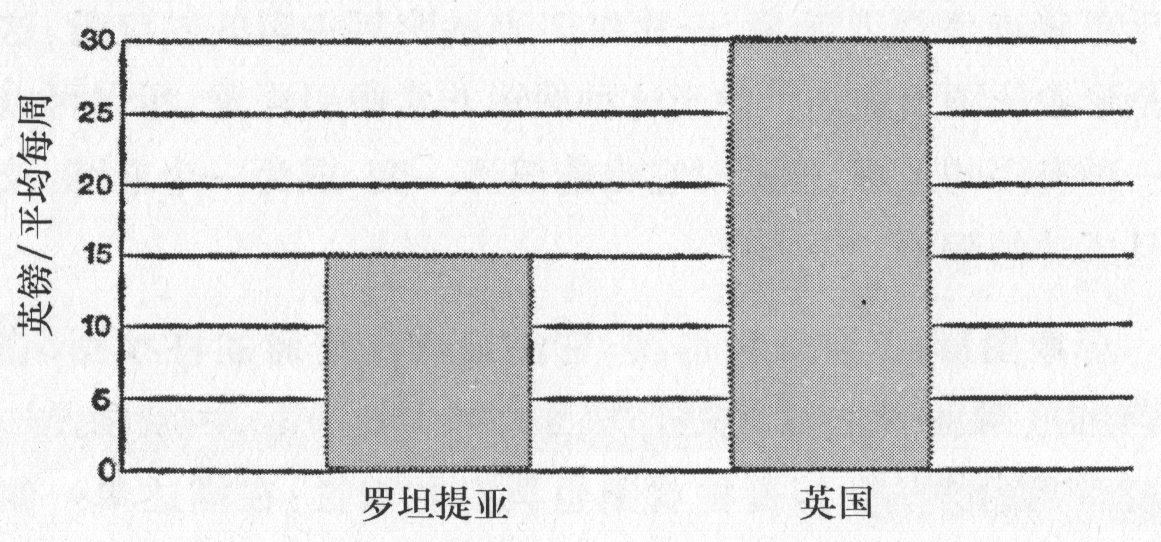
\includegraphics[width=0.9\textwidth]{c4.case.1d.bar.01.png}
  \end{figure}
  \vspace{-1em}
  \begin{block}{解析}
    \begin{itemize}
      \item 清楚且忠于事实的图形——收入是1:2的比例关系,图中两根柱体的比例也是1:2。
      \item 图形并不吸引眼球!——用钱袋来表示收入。
    \end{itemize}
  \end{block}
\end{frame}

\begin{frame}
  \frametitle{案例 | 维度 | 工资}
  \begin{block}{钱袋图}
    画一个钱袋用来表示罗坦提亚人的15英镑,然后再画一个高两倍的钱袋代表英国佬的30英镑。还是1:2的比例……对吗?
  \end{block}
  \vspace{-0.5em}
  \begin{figure}
    \centering
    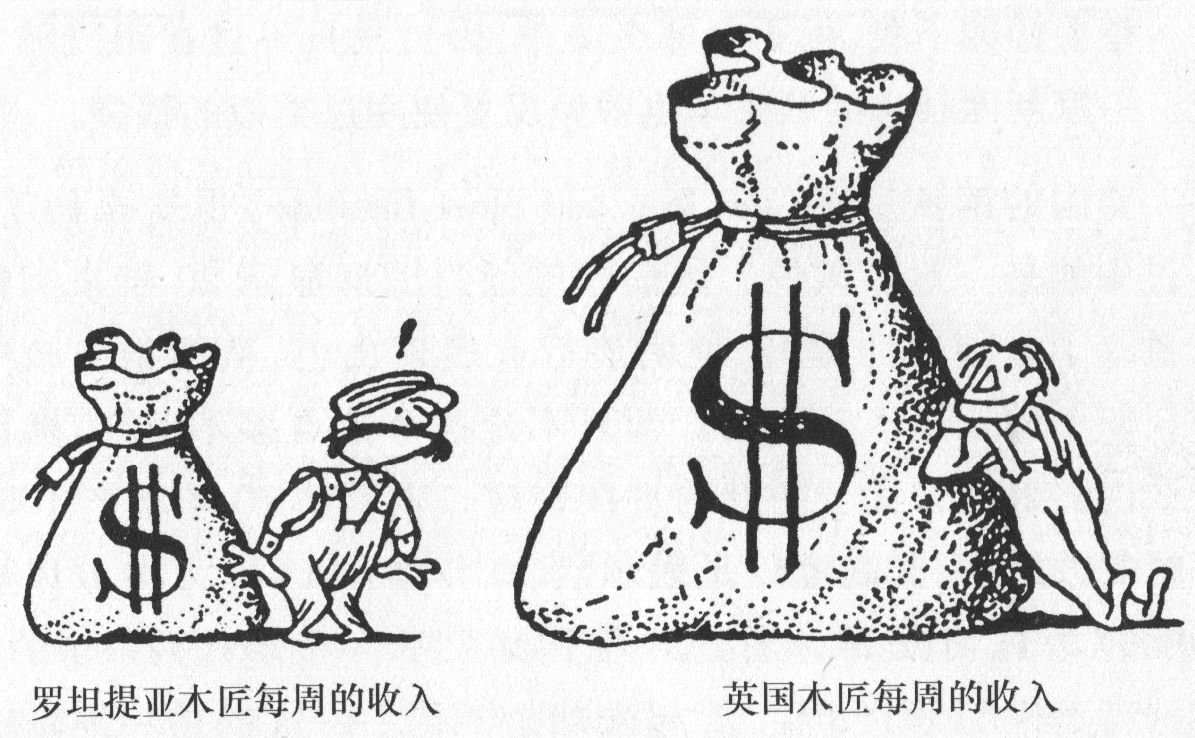
\includegraphics[width=0.75\textwidth]{c4.case.1d.bag.01.png}
  \end{figure}
\end{frame}

\begin{frame}
  \frametitle{案例 | 维度 | 工资}
  \begin{block}{解析}
    \begin{itemize}
      \item 直观的感受——英国佬的收入使得罗坦提亚工人相形见绌。
      \item 奥妙的关键——既然第二个袋子比第一个高一倍,也应该同样宽一倍,那么占用纸张的空间就不是2倍而变成4倍。
      \item 数字全是2:1,但视觉效果却是4:1,而在大多数时候视觉效果起着决定性的作用。
      \item 实际事物往往是三维的——如果一个钱袋里有15英镑,另一个钱袋里面就不仅仅只装了30英镑,而应该是120英镑(15英镑的8倍)!
      \item 明明说的是“2倍”,却最终让你留下了令人震惊的8倍的印象。
    \end{itemize}
  \end{block}
\end{frame}

\begin{frame}
  \frametitle{案例 | 维度 | 收入}
  \begin{figure}
    \centering
    \visible<1->{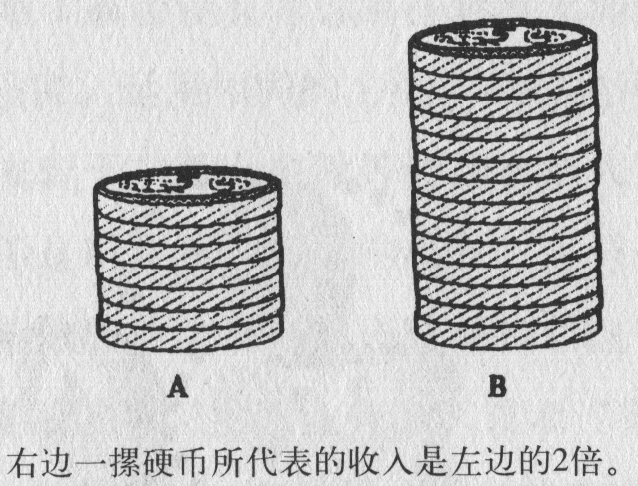
\includegraphics[width=0.23\textwidth]{c4.case.1d.income.01.png}}
    \visible<2->{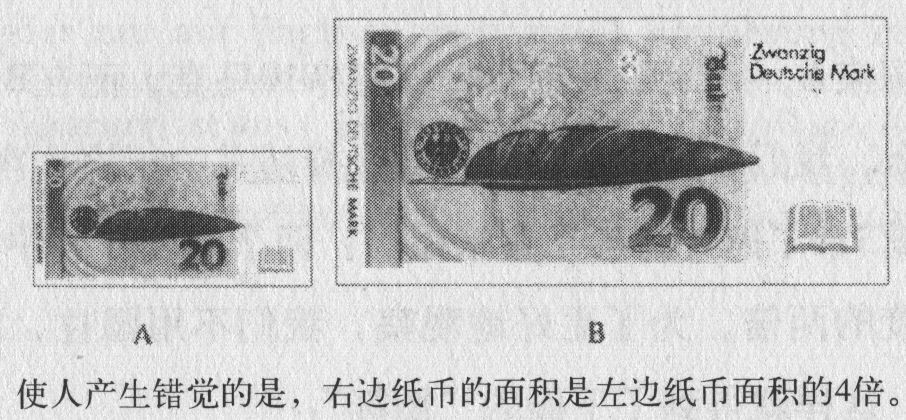
\includegraphics[width=0.38\textwidth]{c4.case.1d.income.02.png}}
    \visible<3->{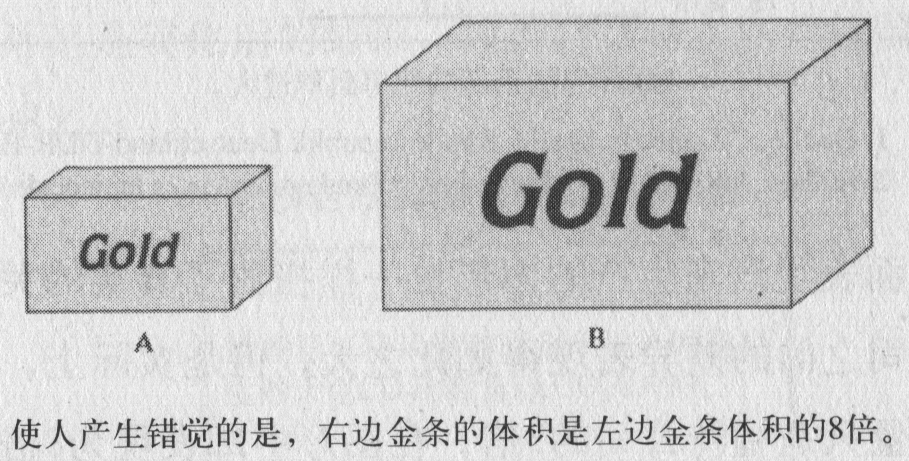
\includegraphics[width=0.35\textwidth]{c4.case.1d.income.03.png}}
  \end{figure}
\end{frame}

\begin{frame}
  \frametitle{案例 | 维度 | 住房面积}
  \begin{block}{联邦德国新州和老州的住房面积}
    \begin{figure}
      \centering
      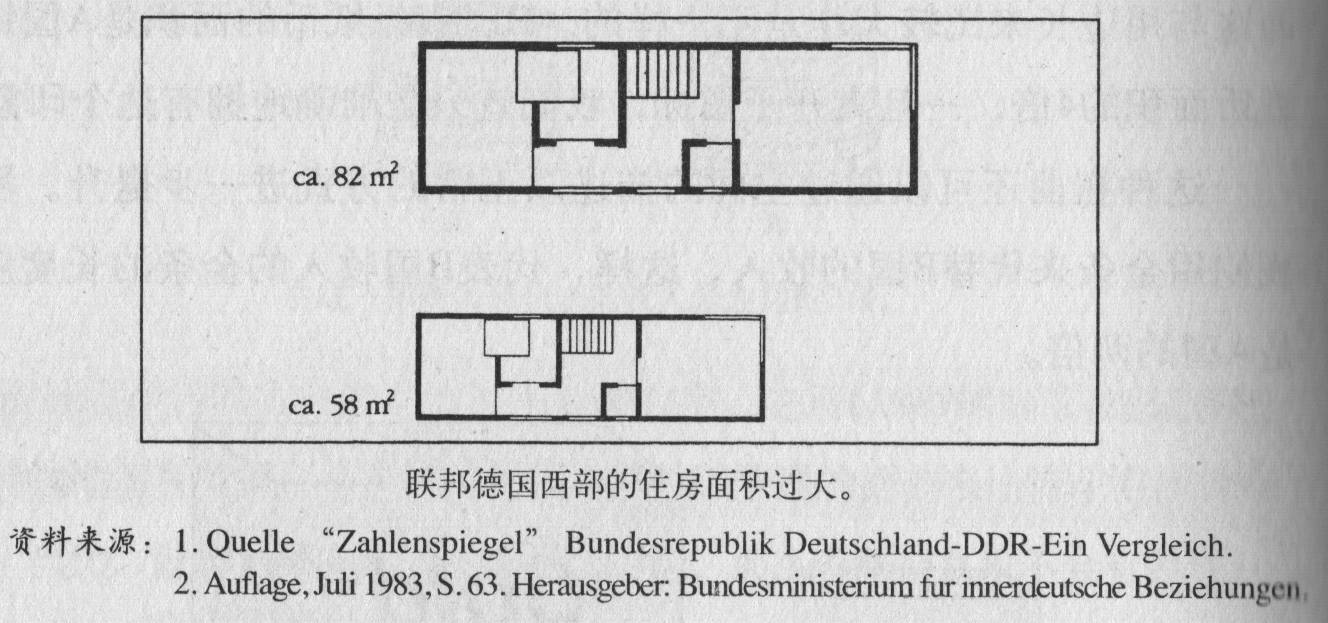
\includegraphics[width=0.9\textwidth]{c4.case.1d.house.01.png}
    \end{figure}
    \vspace{-0.5em}
    不用住房的面积而是用住房的边长来表示,因此,两个平面图的面积就是82:58,而是像实际生活中那样为116:58(住房面积不是多了41\%,而是多了100\%)。
  \end{block}
\end{frame}

\begin{frame}
  \frametitle{案例 | 维度 | 汽车销售数量}
  \begin{figure}
    \centering
    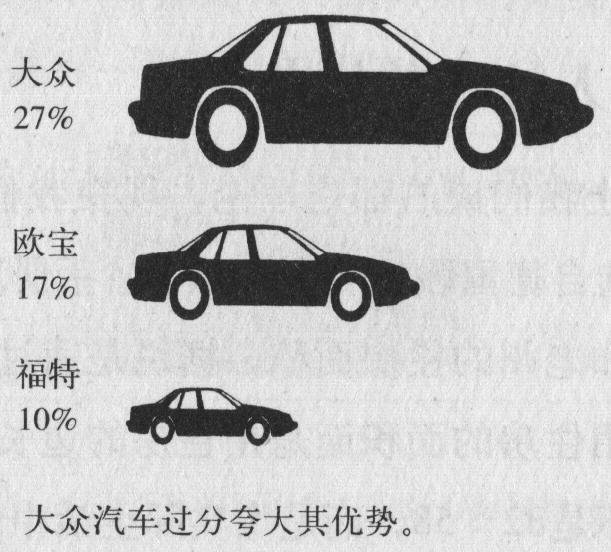
\includegraphics[width=0.7\textwidth]{c4.case.1d.car.01.png}
  \end{figure}
\end{frame}

\begin{frame}
  \frametitle{案例 | 维度 | 二氧化碳排放量}
  \begin{figure}
    \centering
    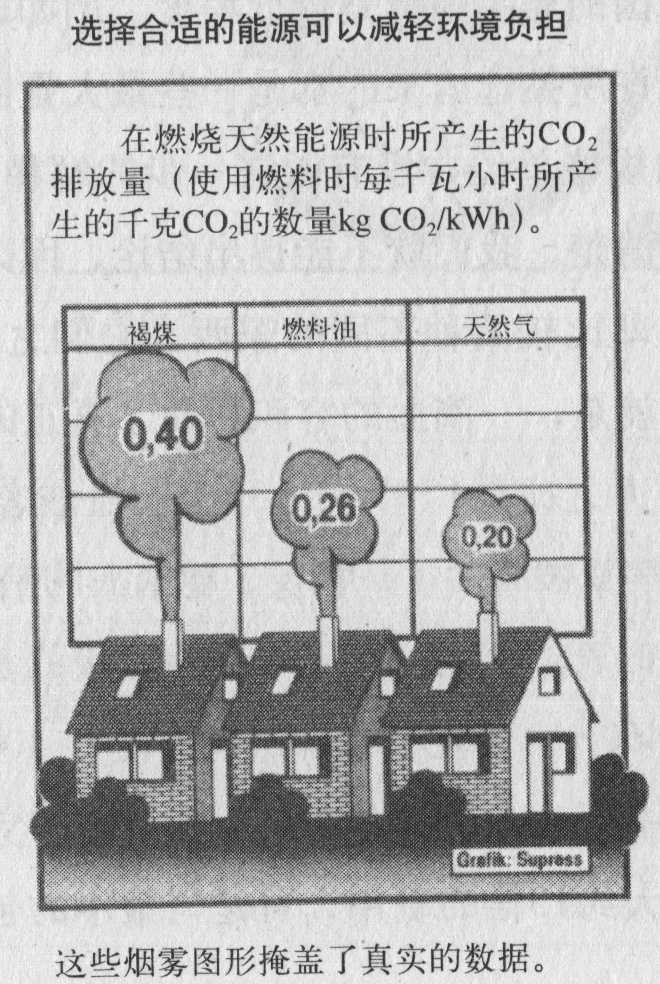
\includegraphics[width=0.43\textwidth]{c4.case.1d.co2.01.png}
  \end{figure}
\end{frame}

\begin{frame}
  \frametitle{案例 | 维度 | 欧盟国中每个就业者的补贴状况}
  \begin{figure}
    \centering
    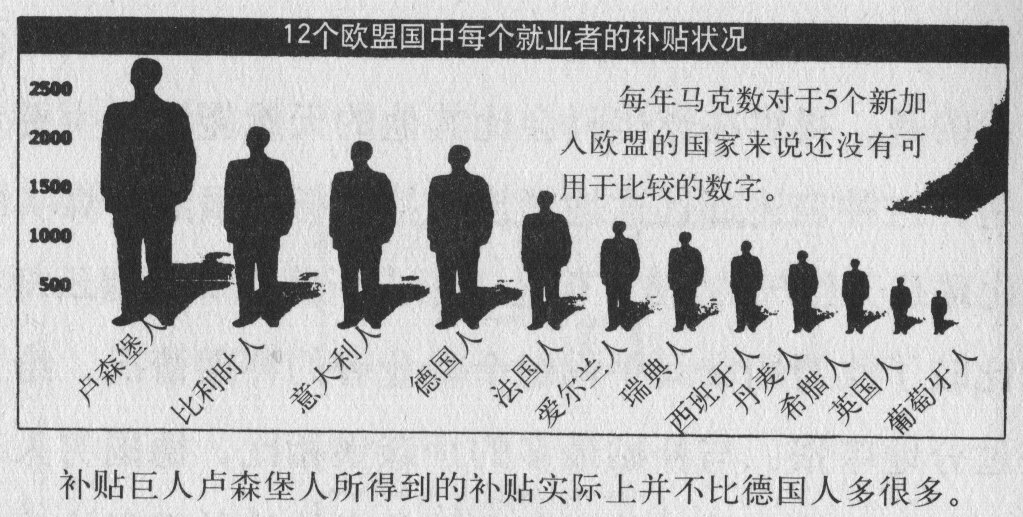
\includegraphics[width=0.9\textwidth]{c4.case.1d.om.01.png}
  \end{figure}
\end{frame}

\begin{frame}
  \frametitle{案例 | 维度 | 药品消费}
  \begin{figure}
    \centering
    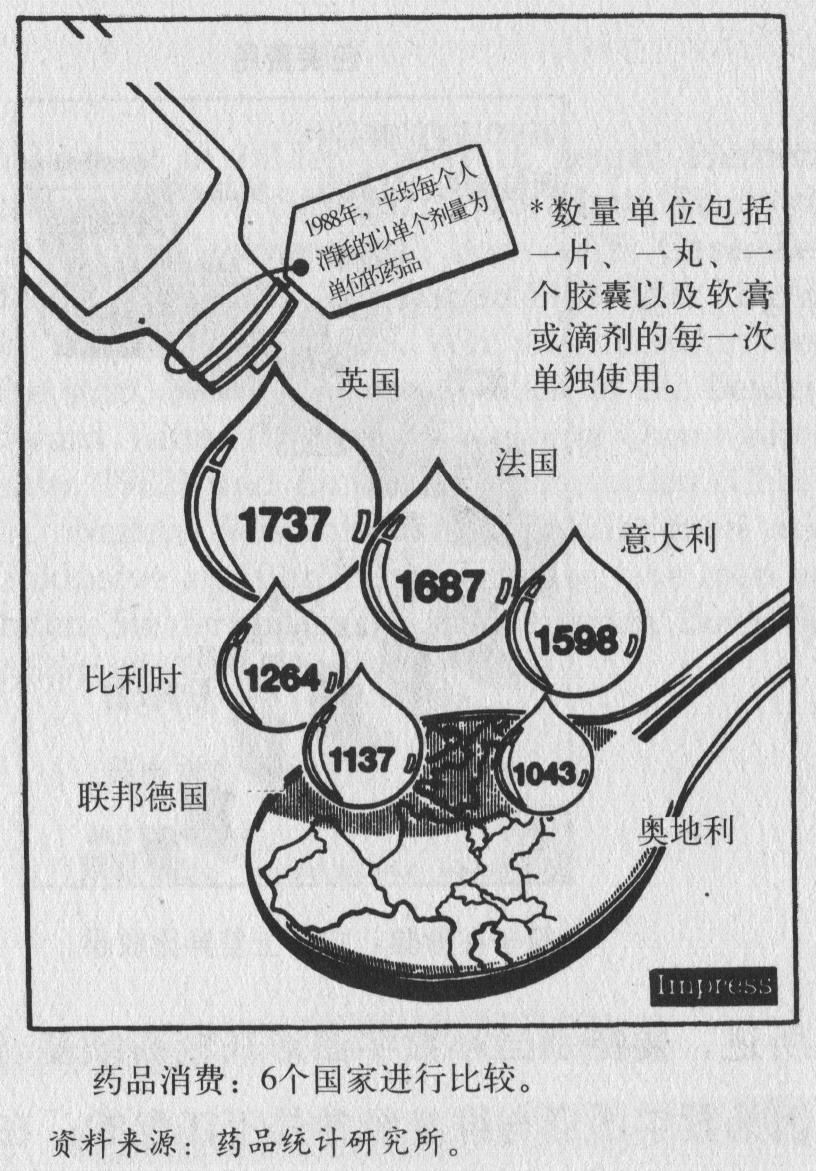
\includegraphics[width=0.45\textwidth]{c4.case.1d.drug.01.png}
  \end{figure}
\end{frame}

\begin{frame}
  \frametitle{案例 | 维度 | 垃圾量}
  \begin{figure}
    \centering
    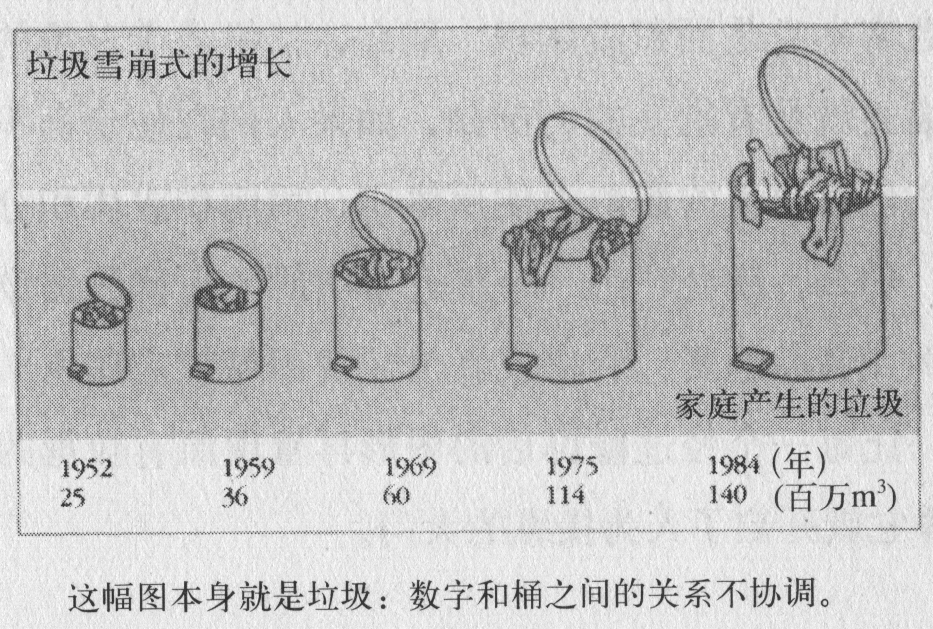
\includegraphics[width=0.9\textwidth]{c4.case.1d.trash.01.png}
  \end{figure}
\end{frame}

\begin{frame}
  \frametitle{案例 | 维度 | 包装费用}
  \begin{figure}
    \centering
    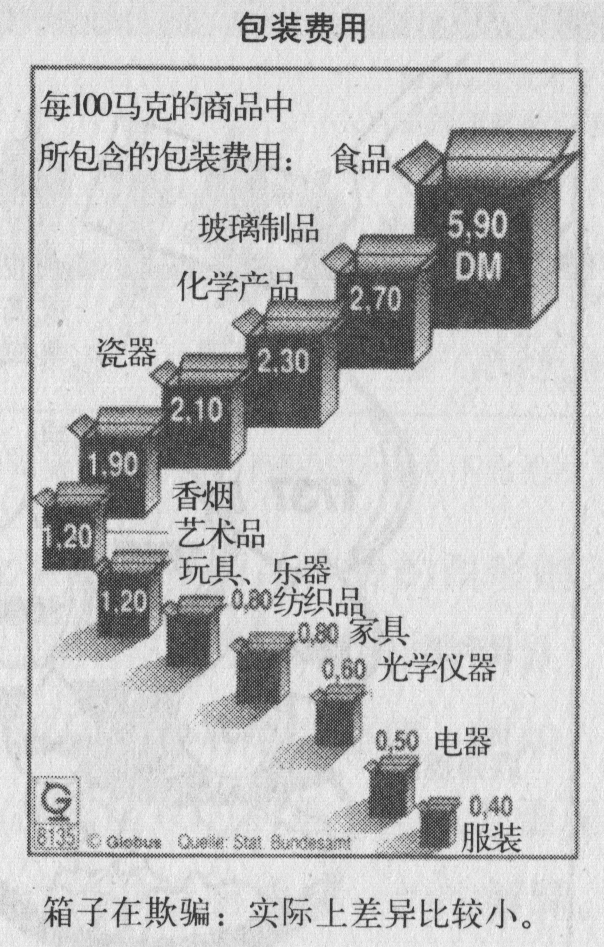
\includegraphics[width=0.4\textwidth]{c4.case.1d.box.01.png}
  \end{figure}
\end{frame}

\begin{frame}
  \frametitle{案例 | 维度 | 钢产量}
  \begin{block}{目的}
    美国钢铁协会希望通过图形显示20年来钢铁产量有了大幅度的提高,说明该行业表现出色,从而指出政府的任何干预都是不必要的。
  \end{block}
  \vspace{-0.5em}
  \begin{figure}
    \centering
    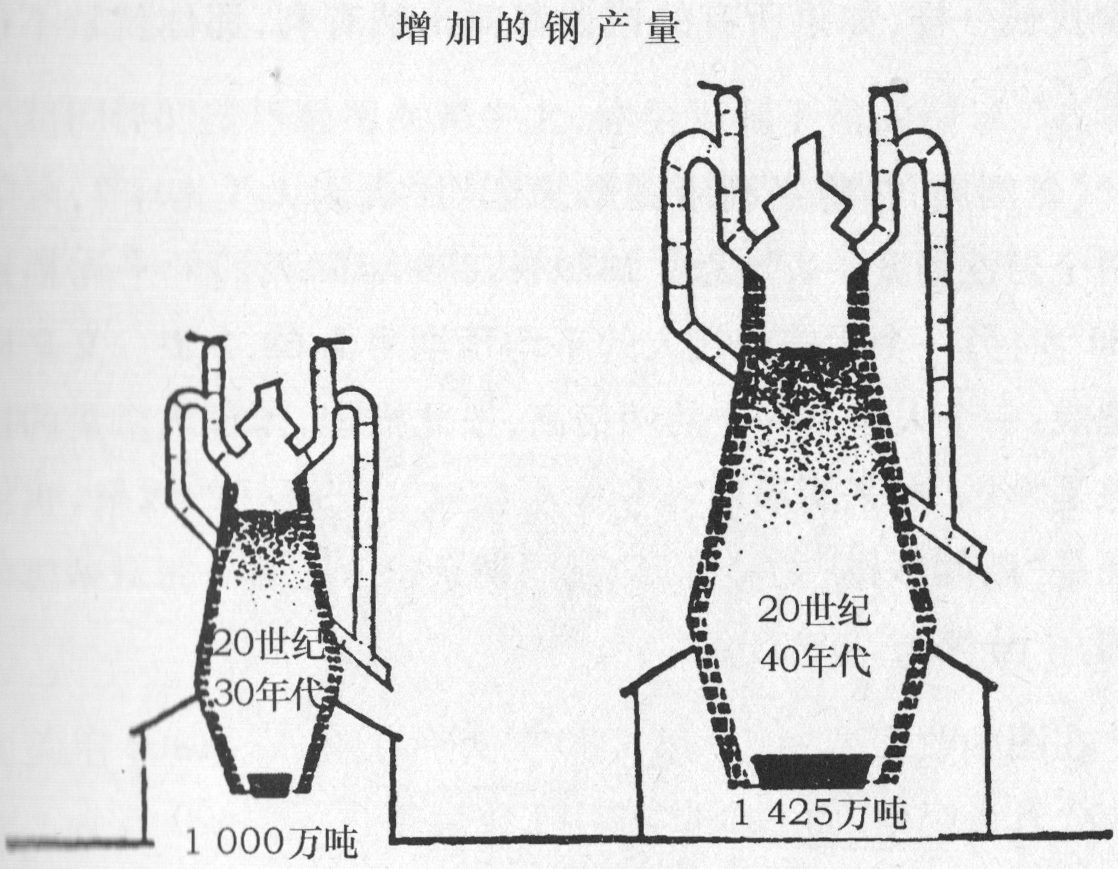
\includegraphics[width=0.6\textwidth]{c4.case.1d.iron.01.png}
  \end{figure}
\end{frame}

\begin{frame}
  \frametitle{案例 | 维度 | 钢产量}
  \begin{block}{解析——变成魔术的算术}
    \begin{itemize}
      \item 表示前10年增产1000万吨的鼓风炉,其高度仅是表示后10年增产1425万吨鼓风炉高度的2/3。但是眼睛看到的两个鼓风炉,一个却是另一个的3倍。嘴上说的是1.5倍,看起来却是3倍。
      \item 从水平上看,第二个鼓风炉似乎“胖些”,其宽度与其邻居的比例失调。
      \item 鼓风炉内的黑色条块,代表这熔化的铁,其长度看上去是10年前的2.5倍。于是,50\%的增长率被画成了150\%的增长率,视觉效果又将其变成1500\%的增长率。
    \end{itemize}
  \end{block}
\end{frame}

\begin{frame}
  \frametitle{案例 | 维度 | 奶牛}
  \begin{figure}
    \centering
    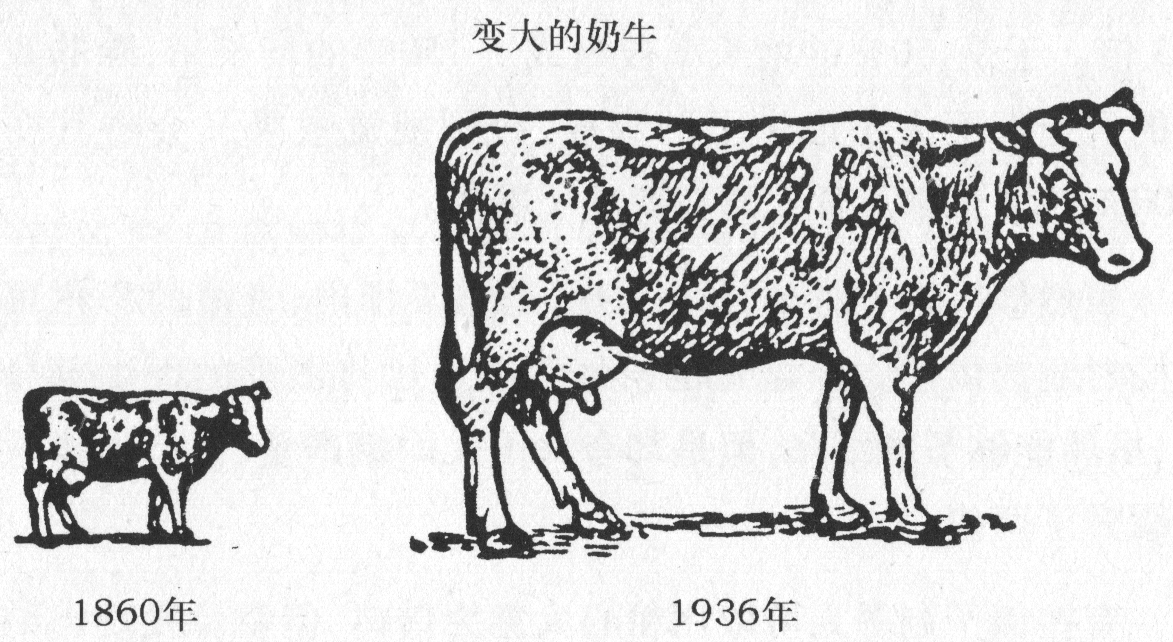
\includegraphics[width=0.8\textwidth]{c4.case.1d.nn.01.png}
  \end{figure}
  \vspace{-1em}
  \pause \pause \pause \pause
  \begin{block}{效果}
    \begin{itemize}
      \item 真实目的:1860年美国只有800万头奶牛,而一个世纪后该数量超过了2500万头。
      \item 实际效果:现在的牛要比以前的牛大得多。
    \end{itemize}
  \end{block}
\end{frame}

\begin{frame}
  \frametitle{案例 | 维度 | 犀牛}
  \begin{figure}
    \centering
    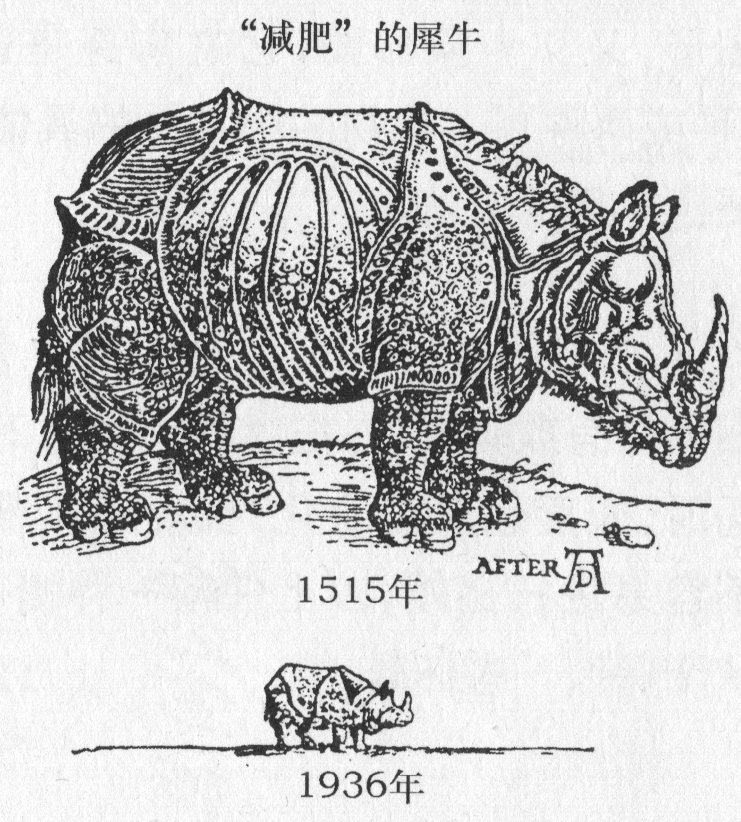
\includegraphics[width=0.55\textwidth]{c4.case.1d.xn.01.png}
  \end{figure}
\end{frame}

\subsection{地理地图}
\begin{frame}
  \frametitle{案例 | 地图 | 世界的中心}
  \begin{block}{哪里是世界的中心?}
    \begin{figure}
      \centering
      \includegraphics[width=0.5\textwidth]{c4.case.world.01.png}\quad
      \includegraphics[width=0.43\textwidth]{c4.case.world.02.png}
    \end{figure}
  \end{block}
\end{frame}

\begin{frame}
  \frametitle{案例 | 地图 | 人口密度图}
  \begin{block}{联邦德国的居民密度}
    \begin{figure}
      \centering
      \includegraphics[width=0.7\textwidth]{c4.case.population.01.png}
    \end{figure}
  \end{block}
\end{frame}

\begin{frame}
  \frametitle{案例 | 地图 | 医生职位}
  \begin{block}{“空的”医生职位}
    \begin{figure}
      \centering
      \includegraphics[width=0.75\textwidth]{c4.case.doctor.01.png}
    \end{figure}
  \end{block}
\end{frame}

